%Auteurs : Nicolas Englebert
\documentclass[british,french,11pt, a4paper]{report}

% Règles de bonne pratiques :
% https://fr.wikibooks.org/wiki/LaTeX/Gestion_des_gros_documents

%%%%%%%%%%%%%%%%
%%% Packages %%%
%%%%%%%%%%%%%%%%

%%% Général %%%
\usepackage[utf8]{inputenc}   
\usepackage[french]{babel}
\usepackage[T1]{fontenc}
\usepackage{mathpazo}
\usepackage{lmodern}
\usepackage{courier}
\usepackage{graphicx}
\usepackage{cancel}

%%% Tableau %%%
\usepackage{tabularx} %Permet d'auto dimensionner les tableaux



%%% Bibliographie %%%
\usepackage[style=alphabetic,backend=bibtex]{biblatex}
\usepackage[autostyle]{csquotes}
\DeclareNameAlias{sortname}{last-first}
\DeclareFieldFormat{url}{\space\url{#1}}
\DeclareNameAlias{labelname}{last-first}
\addbibresource{sample.bib}


%%% Graphiques %%%
\usepackage{tikz}
\usepackage{pgfplots}
\usepackage{circuitikz}

%%% Mise en page %%%
\usepackage{amsmath}
\usepackage{amsfonts}
\usepackage{amssymb}
\usepackage{amsthm}
\usepackage[tt]{titlepic}% Centre le titre
\usepackage{fancyhdr}   % Permet de modifier l'entête & footer
\usepackage{caption}     % Permet d'ajouter des légendes en images sans les mettre en float + dans la marge + ref vers le haut de l'envirronement
\usepackage{wrapfig}
\usepackage{fullpage}
\usepackage{multicol}   % pour les liste sur plusieurs colonnes
\usepackage{subfigure}  % alligne deux images cote a cote
\usepackage{float}      %permet de mettre du texte entre les figures grace a [H]. Génial! 
\usepackage{eso-pic}    % Fond d'écran page de garde
\usepackage{adjustbox}  % Empêche les box de sortir de la page


%%% Math %%%
\usepackage{delarray} % Belles matrices
\usepackage{siunitx}
\sisetup{locale = FR,detect-all}
% Pour mettre siunitx en mode français (virgule plutôt que point etc.)

%%% Codes %%%
\usepackage{listings}
\usepackage[final]{pdfpages} %% Inclusion fichier pdf

%% Reference
\usepackage{hyperref}
\renewcommand*{\figureautorefname}{fig.}
\def\appendixautorefname{annexe}
\def\tableautorefname{tab.}
\renewcommand*{\chapterautorefname}{ch.}




%%%%%%%%%%%%%%%%%
%%% Commandes %%%
%%%%%%%%%%%%%%%%%

%%% Physique %%%
\newcommand{\cst}{\text{cst}}
\newcommand{\D}{\partial}
\newcommand{\E}{\vec E}
\newcommand{\B}{\vec B}
\newcommand{\F}{\vec F}
\newcommand{\modu}[1]{|$#1$|}

%%% Math %%%
\newcommand{\oiint}{\int\!\!\!\!\!\!\! \:\!\subset\!\!\supset\!\!\!\!\!\!\!\int}
\newcommand{\rot}{\text{rot}\,}
\newcommand{\divv}{\text{div}\,}
\newcommand{\phas}[1]{\underline{#1}}
\newcommand{\RE}{\text{Re}}
\newcommand{\ft}{\overset{\mathcal{F}}{\longleftrightarrow}}
\newcommand{\lt}{\overset{\mathcal{L}}{\longleftrightarrow}}




%% Box
\newcommand{\theor}[1]{\adjustbox{minipage=\linewidth-2\fboxsep-2\fboxrule,fbox}{\textsc{Théorème : }#1}}
\newcommand{\defi}[1]{\adjustbox{minipage=\linewidth-2\fboxsep-2\fboxrule,fbox}{\textsc{Définition : }#1}}
\newcommand{\lemme}[1]{\adjustbox{minipage=\linewidth-2\fboxsep-2\fboxrule,fbox}{\textsc{Lemme : }#1}}
\newcommand{\prop}[1]{\adjustbox{minipage=\linewidth-2\fboxsep-2\fboxrule,fbox}{\textsc{Propriété}\\ #1}}
\newcommand{\proposition}[1]{\adjustbox{minipage=\linewidth-2\fboxsep-2\fboxrule,fbox}{\textsc{Proposition}\\#1}}
\newcommand{\retenir}[1]{\adjustbox{minipage=\linewidth-2\fboxsep-2\fboxrule,fbox}{\textbf{\textit{\textsc{A retenir} : }}#1}}
\newcommand{\corollaire}[1]{\ \\\begin{tabular}{||c}
	\begin{minipage}{\textwidth}
		\textsc{Corollaire : } \textit{#1}
	\end{minipage}
	\end{tabular}}
\newcommand{\exemple}[1]{\ \\\begin{tabular}{|c}
	\begin{minipage}{\textwidth}
		\textsc{Exemple : } #1
	\end{minipage}
	\end{tabular}}
    
    

%\pagestyle{headings} % Titre du ch et numéro page dans l'entete
\renewcommand{\proofname}{Démonstration}
\selectlanguage{french}

\addto\captionsfrench{\def\tablename{Tableau}}


%%% Background %%%
\newcommand\BackgroundPic{%
	\put(0,0){%
		\parbox[b][\paperheight]{\paperwidth}{%
			\vfill
			\centering
			
\includegraphics[width=\paperwidth,height=\paperheight,%
			keepaspectratio]{../../Builder/ulb.jpg}%
			\vfill
}}}

%%% Annexes Cedu %%%
%\usepackage{calrsfs}
\DeclareMathAlphabet{\pazocal}{OMS}{zplm}{m}{n}
\usepackage{fourier-orns}

\setlength{\parindent}{0pt} 

%%% Attributs %%%
\newcommand*{\NomduCours}[2]{\def\cours{#1}\def\memo{#2}}
\newcommand*{\auteur}[2]{\def\prenom{#1}\def\nom{#2}}
\newcommand*{\rappeltheo}[2]{\def\rappeltheoprenom{#1}\def\rappeltheonom{#2}}
\newcommand*{\professeur}[2]{\def\pprenom{#1}\def\pnom{#2}}
\newcommand*{\sprofesseur}[2]{\def\spprenom{#1}\def\spnom{#2}}
\newcommand*{\annee}[2]{\def\adebut{#1}\def\afin{#2}}
\graphicspath{{img/}}

% Attributs
\NomduCours{Économie politique et sociale}{GEST-H-200}
\auteur{Enes}{Ulusoy}
\professeur{Michel}{Allé}
\annee{2014}{2015}

% Document
\begin{document}
	\def\equationautorefname~#1\null{%
		(#1)\null
	}
	
	
	%%%%%%%%%%%%%%%%%
	% Préliminaires %
	%%%%%%%%%%%%%%%%%
	\cleardoublepage
	%\@mainmatterfalse
	\pagenumbering{roman}
	
	\AddToShipoutPicture*{\BackgroundPic}

\begin{titlepage}
	\begin{center}	
			
		\newcommand{\HRule}{\rule{\linewidth}{0.5mm}}   			            %Titre en gros
		
\includegraphics[scale=0.11]{../../Builder/titlepage/logo.jpg}~\\[1cm]				%Logo
			
			\textsc{\LARGE Université Libre de Bruxelles}\\[1.5cm]
			\textsc{\Large Synthèse}\\[0.5cm]
			
			\HRule \\[0.4cm]
			{ \huge \bfseries \cours \ \\\memo \\[0.4cm] }
			
			
			\HRule \\[1.5cm]
			\begin{minipage}[t]{0.6\textwidth}
				\begin{flushleft}%\large
					\emph{Auteur :}\\
					\mbox{\prenom~\textsc{\nom}}\\
					\ifdefined\nnom
					\ \\
					\emph{Notes :}\\
					\mbox{\nprenom~\textsc{\nnom}}\\
					\fi
					\ifdefined\rappeltheonom
					\ \\
					\emph{Rappels théoriques :}\\
					\mbox{\rappeltheoprenom~\textsc{\rappeltheonom}}
					\fi 
				\end{flushleft}
			\end{minipage}
			\begin{minipage}[t]{0.25\textwidth}
				%\begin{flushright}
				%\large
				\emph{Professeur :}\\
				\mbox{\pprenom~\textsc{\pnom}}
				\ifdefined\spprenom
				\\ \mbox{\spprenom~\textsc{\spnom}} \\
				\fi
				%\end{flushright}
			\end{minipage}
			
			\vfill
			
			% Bottom of the page
			{\large Année \adebut~-~\afin}
			
		\end{center}
	\end{titlepage}

	\chapter*{Appel à contribution}
\subsection*{Synthèse Open Source}
\begin{wrapfigure}[5]{l}{4.5cm}
	
\includegraphics[scale=0.5]{../../Builder/git.png}
\end{wrapfigure}
Ce document est grandement inspiré de l’excellent cours donné 
par \pprenom~\pnom\	
\ifdefined\spprenom
et\ \spprenom~\spnom\ 
\fi
 à l’EPB (École Polytechnique de Bruxelles), faculté de l’ULB (Université 
Libre de Bruxelles). Il est écrit par les auteurs susnommés avec l’aide de tous les autres étudiants 
et votre aide est la bienvenue ! En effet, il y a toujours moyen de l’améliorer surtout que si le 
cours change, la synthèse doit être changée en conséquence. On peut retrouver le code source à l’adresse 
suivante
\begin{center}
	\url{https://github.com/nenglebert/Syntheses}
\end{center}\ \\
Pour contribuer à cette synthèse, il vous suffira de créer un compte sur \textit{Github.com}. De
légères modifications (petites coquilles, orthographe, ...) peuvent directement être faites sur le
site ! Vous avez vu une petite faute ? Si oui, la corriger de cette façon ne prendra que quelques 
secondes, une bonne raison de le faire ! \\
\\
Pour de plus longues modifications, il est intéressant de disposer des fichiers : il vous 
faudra pour cela installer \LaTeX, mais aussi \textit{git}. Si cela pose problème, nous sommes 
évidemment ouverts à des contributeurs envoyant leur changement par mail ou n’importe quel autre 
moyen.\\
\\
Le lien donné ci-dessus contient aussi le \texttt{README} contient de plus amples informations, 
vous êtes invités à le lire si vous voulez faire avancer ce projet ! 

\subsection*{Licence Creative Commons}
\begin{wrapfigure}[3]{r}{2.8cm}
	\vspace{-5mm}
	
\includegraphics[scale=0.17]{../../Builder/CC}
\end{wrapfigure}
Le contenu de ce document est sous la licence Creative Commons : \textit{Attribution-NonCommercial-ShareAlike 
4.0 International (CC BY-NC-SA 4.0)}. Celle-ci vous autorise à l'exploiter pleinement, compte-
tenu de trois choses :
\begin{enumerate}
	\item \textit{Attribution} ; si vous utilisez/modifiez ce document vous devez signaler le(s) nom(s)
	      de(s) auteur(s).
	\item \textit{Non Commercial} ; interdiction de tirer un profit commercial de l’œuvre sans 
	      autorisation de l'auteur 
	\item \textit{Share alike} ;  partage de l’œuvre, avec obligation de rediffuser selon la même 
	      licence ou une licence similaire
\end{enumerate}
Si vous voulez en savoir plus sur cette licence :
\begin{center}
	\url{http://creativecommons.org/licenses/by-nc-sa/4.0/}
\end{center}

\begin{flushright}
	\textbf{Merci ! }
\end{flushright}
	\tableofcontents
	%Si abstract, \input ici
	
	%%%%%%%%%%%%%%%%%%%%%
	% Contenu principal %
	%%%%%%%%%%%%%%%%%%%%%
	\cleardoublepage
	% \@mainmattertrue
	\pagenumbering{arabic}
	%%%%%%%%%%%%%%%%%%%%%%%
%%      Lecon 1      %%
%%%%%%%%%%%%%%%%%%%%%%%

\chapter{Les origines de la crise : \\ Les prêts hypothécaires "subprimes"}
Comme beaucoup le savent, un prêt hypothécaire est un prêt accordé pour un bien immobilier en garantissant le remboursement par ce bien. En effet, en cas d'impossibilité de remboursement, la banque met la main sur le bien. C'est sur le terme "subprime" que nous allons nous intéressé dans ce chapitre qui sera expliqué dans son contexte.

\section{Ca craque une première fois}
\textbf{Ralph Cioffi} est un gestionnaire "génial" de fonds. Il collecte beaucoup d'argent chez les investisseurs et investit cet argent dans des actifs (actions, immeubles, ...). Puisqu'un gestionnaire de fond est rémunéré selon les montants gérés et sur la rentabilité, il s'efforce d'obtenir le meilleur rendement (retour d'argent) avec un risque faible (peu d'argent). Pour améliorer ce rendement, \textbf{on s'endette au maximum !} \\
D'un autre côté, les banques qui prêtent veulent être sûres de retrouver leur mise \footnote{La banque \textbf{Merrill Lynch} a prêté beaucoup d'argent au fonds géré par Ralph Cioffi.}. Pour cela, elles vérifient régulièrement si la valeur des actifs est supérieure aux dettes. Si ce n'est pas le cas, elle procède à un \textbf{appel de marge} (demande de l'argent au fonds). \\

Pour financer l'appel de marge, on a, dans l'ordre, trois chances :
\begin{enumerate}
\item \textbf{Utiliser le cash disponible dans le fonds.}
\item \textbf{Faire appel aux investisseurs.}
\item \textbf{Vendre des actifs.}
\end{enumerate}

Ce qui s'est passé en 2007, c'est que justement il n'y avait plus de cash, les investisseurs refusaient d'investir et les biens ne se vendaient pas ! De ce fait, les fonds étaient virtuellement en faillite. \\

\section{Les subprimes}
Mais comment en est-on arrivé à avoir des actifs invendables ? C'est à cause des financiers : 

\begin{enumerate}
\item \textbf{La Finance est modélisée}\\
On était capable de mettre tous les risques en équation et donc on pensait les contrôler. 

\item \textbf{La Finance n'est pas régulée}\\
On prêtait et empruntait sans trop de difficultés et sans règles.

\item \textbf{La Finance est organisée pour prêter le plus possible}\\
Si on a du cash, au plus on prête, au plus le \textbf{bonus} (grâce aux intérêts) sera élevé. Donc on prêtait à tout le monde, qu'il soit CEO \footnote{Chief Executive Officer.} ou employé de guichet.
\end{enumerate}
 
On prêtait donc à presque tout le monde pour acquérir un logement et c'est ce que l'on appelle les \textbf{subprimes}. Ce système fait plaisir aux individus mais aussi à l'économie (l'économie tourne). Les financiers avaient pour hypothèse que \textbf{le prix de l'immobilier ne cesserait d'augmenter quoiqu'il se passe}. Et bein quand c'est le contraire qui s'est passé, ça a fait mal.

\section{Comparaison des différents systèmes de prêt}
Une comparaison entre les différents prêt hypothécaires est disponible à partir du \textbf{slide 8} dans le cours mais voici un bref résumé :

\begin{itemize}
\item \textbf{Prêt hypothécaire classique (taux fixe)}\\
La banque ne prête que 80 \% de la valeur du bien, les 20 \% devant être un apport personnel. Pour un taux fixe et un revenu de ménage mensuel moyen (2700 euro), le ménage devra rembourser environ 47 \% de son salaire mensuel, ce qui est assez lourd. Mais si le salaire monte (3400 euro), on peut diminuer à 38 \%. 

\item \textbf{Prêt hypothécaire à taux variable}\\
Dans les mêmes conditions, le taux qui est plus faible que le fixe à la base peut soit augmenter, soit diminuer. Dans le cas où le taux diminue, c'est plus avantageux au niveau du remboursement. Par contre dans le cas où le taux augmente, on se fait avoir. C'est pire si le salaire moyen n'augmente pas après quelques années et je ne parle même pas du cas où le salaire diminuerai ! Aujourd'hui, les taux sont tellement bas qu'il est préférable de prendre un taux fixe.

\item \textbf{Prêt hypothécaire aux USA (taux variable et pas de limite à la quote part des revenus)}\\
Dans ce modèle, la banque prête la totalité de la valeur du bien. Si le taux augmente avec le temps et que le salaire reste inchangé, la part de remboursement commence aux environ de 65 \% et peut atteindre jusque 92 \%. Il y a donc un réel risque de \textbf{faillite personnel} dans ce système !

\item \textbf{Prêt hypothécaire aux USA (Quotité de 120 \% et "Negative amortization")}\\
Dans ce modèle la banque va non seuelement prêter la totalité de la somme, mais elle donne aussi 20 \% de cash en plus pour usage personnel (trop d'osey). De plus, pendant 5 ans le client ne devra rembourser que les intérêt (remboursement faible) ce qui donne un remboursement d'à peu près 50 \% du salaire. Cependant, après ces 5 ans, quand on commence à payer tout le prêt, si on a de la chance et que le salaire augmente, on aura un remboursement d'environ 80 \%. Si le salaire reste fixe ou qu'il diminue, alors on peut faire ses prières parce qu'on dépassera les 100 \% !
\end{itemize}


\section{Risque considéré comme faible par les banquiers}
Puisqu'on prête plus, le banquier aura plus de comission et sera gagnant. Celui qui emprunte pourra consommer plus et ainsi doper l'économie tout en étant propriétaire de logement. \\
Comme précisé plus haut, les banquiers font l'hypothèse que le prix de l'immobilier ne fera qu'augmenter. Si jamais il y a des problèmes, ce n'est pas grâve puisqu'ils récupère le bien et se fait encore plus d'argent en la revendant.\\

\begin{center}
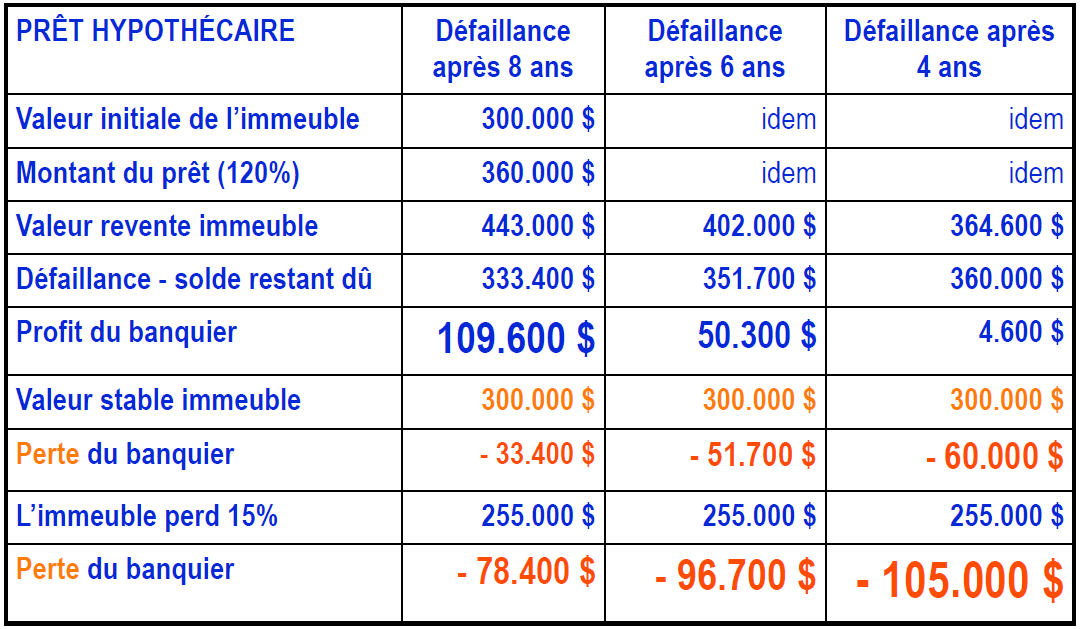
\includegraphics[scale=0.4]{1}
\end{center}

Sur la figure ci-dessus, on peut voir que le banquier gagne d'autant plus que la défaillance arrive tard. Bien sûr, ce n'est le cas que lorsque les prix montent. En effet, si la valeur du bien reste constant, le banquier perd d'office de l'argent (puisqu'il prête 120 \%). Si jamais la valeur du bien diminue, c'est la dégringolade.

	%%%%%%%%%%%%%%%%%%%%%%%
%%      Lecon 2      %%
%%%%%%%%%%%%%%%%%%%%%%%

\chapter{Des subprimes à Fortis : La contamination du système financier mondial}
\section{Marché immobilier aux USA}
\begin{wrapfigure}[9]{l}{8cm}
	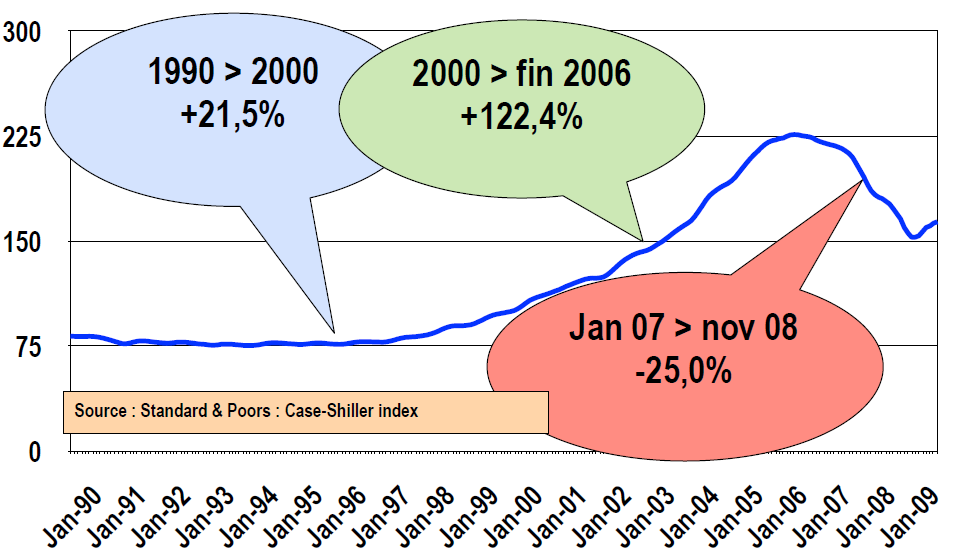
\includegraphics[scale=0.3]{2}
\end{wrapfigure}
\ \\ Comme on peut le voir selon \textbf{l'indice Case-Shiller} \footnote{Outil de mesure de la valeur de l'immobilier important.}, pendant 10 ans la valeur de l'immobilier reste stable. S'en suit une période de 4 ans où la valeur de l'immobilier explose pour finir en chute libre. Les deux premières étapes s'étendent sur une longue durée mais la chute se manifeste par la perte de 25\% de valeur en $\pm$ 1 an !

\begin{wrapfigure}[10]{l}{8cm}
	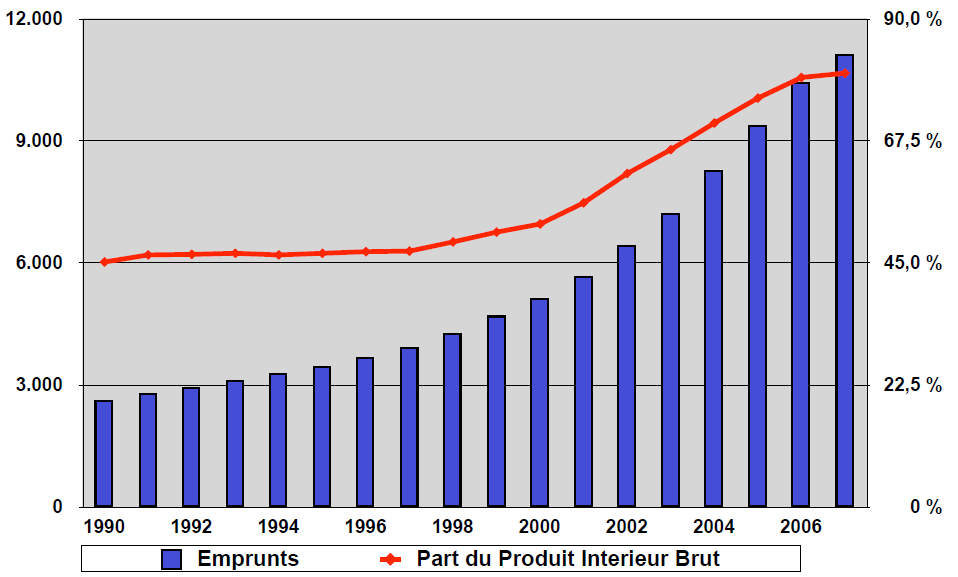
\includegraphics[scale=0.3]{3}
\end{wrapfigure}
\ \\ Si on analyse l'évolution des emprunts durant cette période, on peut constater qu'on a réussi à refiler de plus en plus de crédit. Ceci ravi les banquiers qui ont beaucoup d'argent à distribuer. On observe aussi une explosion de l'emprunt aux alentours de 2002 mais en contre partie, on peut voir que les emprunts ont atteint les 90\% du PIB et donc que celles-ci pèsent sur les ménages. 

\section{L'effet de levier}
On avait vu au premier chapitre que l'objectif de tout investisseur était de maximiser la rentabilité de son investissement. Pour ça, il va donc faire attention non seulement aux \textbf{revenus} (loyer, intérêt, ...) mais il va aussi faire attention à ce que la valeur de revente soit plus élevée \textbf{(plus-value)}. Cependant, selon la loi de la finance (c'est démontrable), une rentabilité élevée signifie un risque élevé. Et donc l'investisseur va essayer de maximiser la rentabilité et minimiser le risque. Pour ça, il a le principe de \textbf{effet levier} :

\begin{wrapfigure}[10]{l}{9cm}
	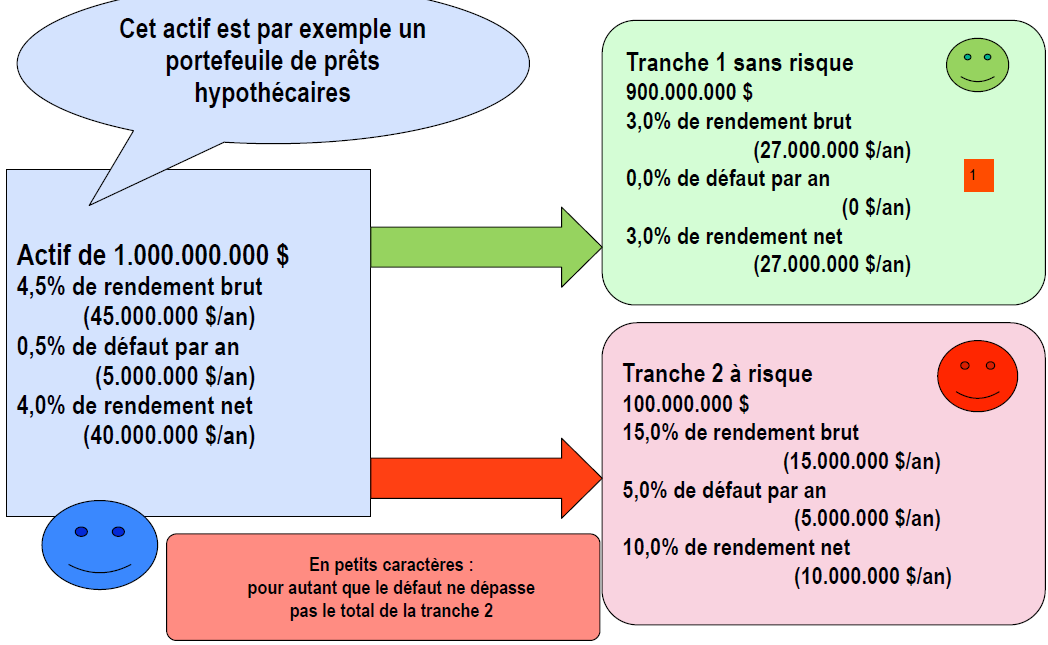
\includegraphics[scale=0.3]{4}
\end{wrapfigure}
Le principe est simple, considérons un investisseurs disposant d'une grande somme d'argent. Il va investir la totalité et aura un revenu brut mais aussi un certain défaut parce qu'il est possible que quelqu'un ne puisse pas rembourser à temps. Pour minimiser le risque et maximiser le gain, il divise le capital en 2 tranches :
\\
\begin{enumerate}
	\item Une première tranche qui consiste en 90\% du capital et qui sera investit sans risque (on considère que c'est garantit) mais avec un gain faible.
	      
	\item Une deuxième tranche qui constitue le reste du capital qui est investit à haut risque et donc qui rapportera gros. 
\end{enumerate}
Donc tout le monde est gagnant et tout le monde est content. 

\section{Innovation financière}
Pour appliquer à fond l'effet de levier, on invente les \textbf{CMO} (Collateralized Mortgage Obligations - 1983) \footnote{Emprunts couverts par des prêts hypothécaires mis en gage.} et \textbf{CDO} (Collateralized Debt Obligations - 1987) \footnote{Emprunts couverts par tout type de dette mises en gage.}. De plus, on découpe le porte feuille en de très nombreuses tranches de risque (comme en haut). Ceci change complètement le métier du crédit parce qu'avant, une seule institution se chargeait de toutes les fonctions (suivi du crédit, ...), la banque intégrée. Mais avec ces pratiques, différentes institutions gèrent différentes fonctions. Ceux-ci sont repris dans le tableau ci-dessous avec leurs conséquences à côté.

\begin{center}
	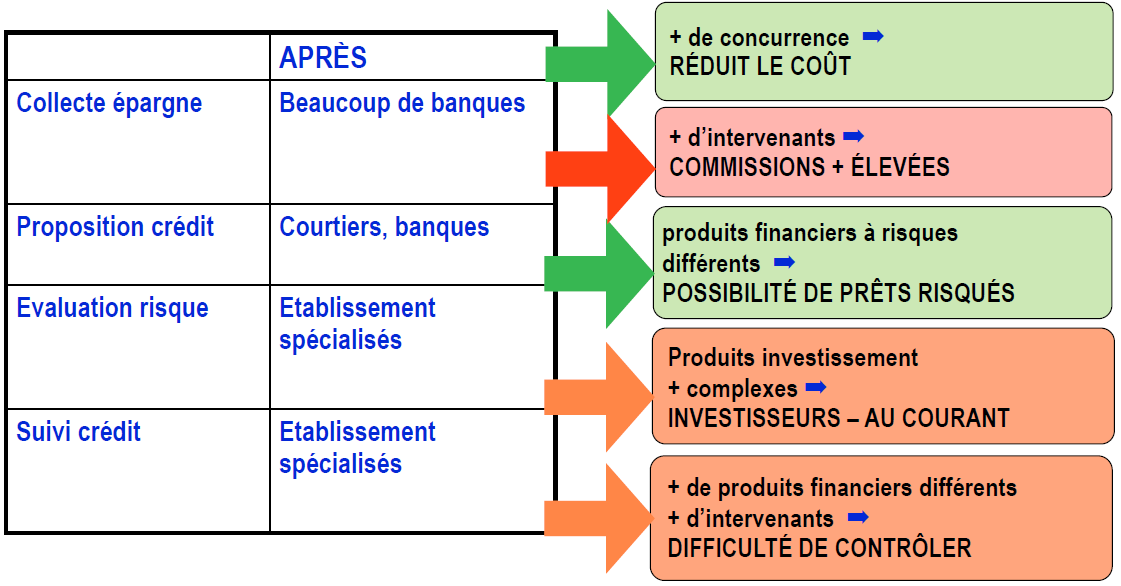
\includegraphics[scale=0.4]{5}
\end{center}

On voit donc qu'en fait on commence à perdre le contrôle sur la finance en raison de cette division. 

\section{Le boom immobilier américain}
Comme on le sait déjà, il y a eu, vers les années 50', une migration massive de la campagnes vers les villes (en Europe et USA). En Asie, elle est venu plus tard, vers les années 90'. Après ce mouvement, il y a eu une certaine migration vers les banlieues\footnote{"Nostalgie des banlieues"} vers les années 70'. Ajoutons à cela, l'explosion démographique entre 1940-45 en Europe et aux USA. \footnote{En gros tous les batards de la guerre ... "Baby boom"}. Mais aux USA, on a encore un phénomène qui stimule l'immobilier qui est la finance. En effet, comme on l'a vu, il y a une offre abondante des banques avec des taux d'intérêts faible. Puisque les ménages n'ont pas vu leur salaire augmenté, on a anticipé la croissance à l'aide d'un principe appelé \textbf{Irrational exubérence} qui est un principe très optimiste sur l'avenir. Cette notion est illustrée sur la figure ci-dessous.

\begin{center}
	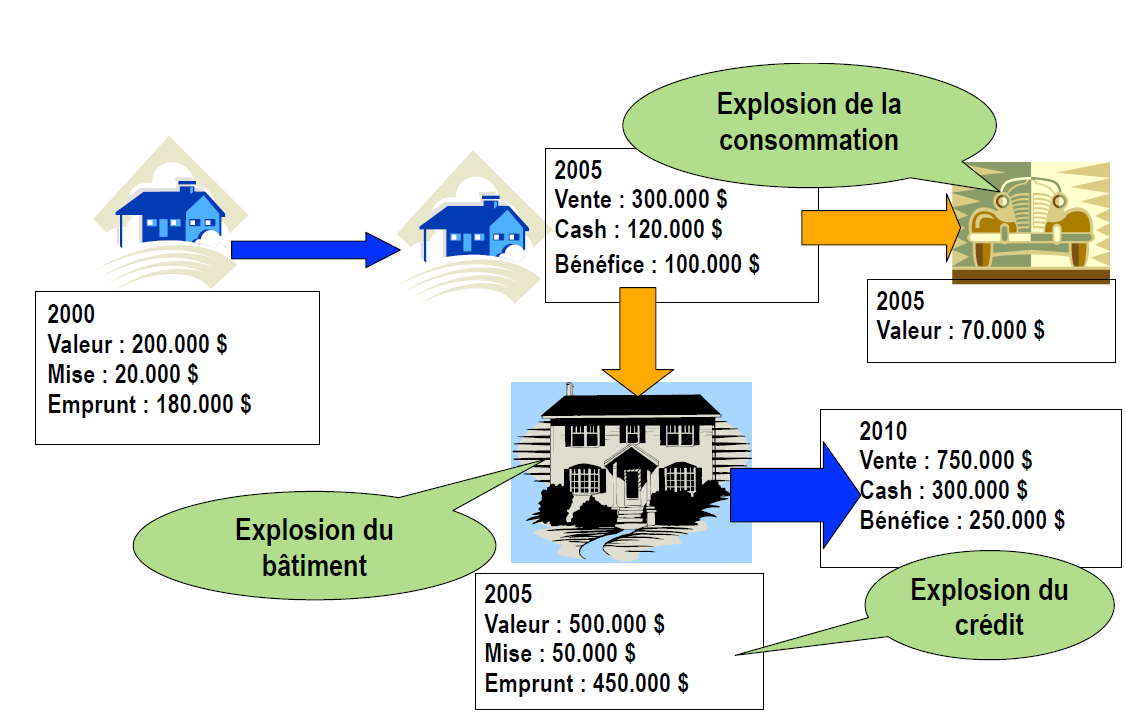
\includegraphics[scale=0.4]{6}
\end{center} 

C'est optimiste car on suppose que la valeur de l'immobilier ne fera qu'augmenter et donc on commence avec petit, ça prend de la valeur, on vend, on a gagné de l'argent donc on peut viser plus grand (plus grand crédit) et dépenser son argent dans d'autre produits et la roue tourne.

\section{Nouvelles innovations financières}
Cependant, si la demande ne suit pas, c'est à dire si les gens n'empruntent pas, ça ne va pas ! C'est pour ça qu'est apparu différentes facilités : taux variable, pas de remboursement du capital ou des intérêts\footnote{"Interest only mortgage"}, options de payement flexible \footnote{Principale remboursé si possible.}, on ne fait plus très attention à la valeur du bien, aux revenus ou au budget du ménage (sub-prime), on peut même aller jusqu'à ne plus faire d'enquête (Alt-A) et on instaure les prêts de longues durées (40 ans et plus) ainsi que les \textbf{emprunts inversé} \footnote{Lorsqu'on décède, on cède le bien à la banque.}. 
\\\\
Tout ceci a pour conséquence que l'immobilier progrèsse très bien (de 122 \% de 2000 à 2006) mais l'innovation financière fait en sorte que les sub-primes et Alt-A prennent une place de plus en plus importante dans le crédit (laisser-aller progressif). 
\\\\
Pour finir, l'effet de levier peut évoluer en \textbf{Hedge Funds} qui ne sont rien d'autres que des fonds à effet de levier maximum. "Hedging" signifie en finance un instrument de sauvegarde ou de protection contre les limites de risque. Il s'agit, par exemple, d'un produit financier qui protège contre les augmentations de taux d'intérêt au-delà de certaines limites. Le principe consiste, par exemple, à investir 100 euro mais on emprunte 400 euro à la banque pour investir 500 euro. De cette manière, on utilise là une première fois l'effet levier. On peut aussi iinvestir dans les CDO qui eux aussi utilise l'effet levier ! On a donc un double effet levier. Les bénnéfices sont donc beaucoup plus élevés mais au détriment du risque qui prend une plus grande importance également. 
\\\\
On a donc là fait le bilan de toutes les innovations : 
Les instruments de "Hedging" offrent souvent, pour la même mise de fonds, des perspectives de rendement plus élevées. avec, à la clé, plus de risques (ce dont les investisseurs ne sont pas toujours conscients).
Les "Hedge Funds" investissent en principe majoritairement dans ce type de produit.
Quand je dis utiliser soi-même l'effet de levier, j'entends que généralement les "Hedge Funds" s'endettent. En outre ils investissement fréquemment dans des produits de type CDO qui utilisent à leur tour l'effet de levier ! Il y a donc double effet de levier
\begin{enumerate}
	\item \textbf{Sub-prime} : on a prêté massivement sans se soucier du remboursement.
	      
	\item \textbf{Effet de levier} : on donne du haut rendement aux emprunts risqués et on vend, comme sans risque, la grande masse des emprunts. 
	      
	\item \textbf{CDO} : les produits mis en gages sont de pllus en plus sophistiqué et transparents (j'imagine que ça veut dire que c'est plus difficile à vendre).
	      
	\item \textbf{Hedge Fund} : les investisseurs se sont endettés à leur tour pour acheter des CDO et donc faire leur propre effet de levier.
\end{enumerate}

\section{Déclin}
\subsection{Ralph Cioffi}
Si on revient en juin 2007, ça craque pour deux fonds qu'il gère. Les fonds, investits en CDO appartiennent à la banque \textbf{Bear Stearns}. Ils empruntent donc chez Merril Lynch. Puis ça s'effondre ! La valeur des CDO diminue et Merril Lynch procède à un appel de marge de 145 millions de dollars. Bear Stearns n'arrive pas à vendre les CDO et Merril les réquisitionne. Sauf que lui non plus n'arrive pas à les vendre. Bear Stearns licencie Cioffi et réinjecte 3,2 miliards de dollars. \\
En août et septembre, plusieurs grandes banques annoncent des pertes sur les sub-primes (20 milliards). \\
En novembre, ces estimations de pertes ont explosé ! On est passé de 20 milliards à 400 ou 500 milliards de dollars ! \\
Un analyste a demandé à Garry Grittenden si la vague de dépréciations étaient finies. La réponse a été très incertaine. Ceci montre que la situation n'est plus sous contrôle. 

\subsection{Piliers de la banque}
Le pilier d'une banque c'est bien sûr la confiance. Cette confiance doit être attribué par : 
\begin{enumerate}
	\item \textbf{Les épargnants} : c'est des clients que vient l'argent, donc source primaire de financement.
	\item \textbf{Les autres banquiers} : il y a des échanges interbancaires quotidiens.
	\item \textbf{Les actionnaires} : qui investissent dans la banque et qui sont souvent épargnants.
	\item \textbf{Le personnel} : qui sont souvent aussi actionnaires et épargnants. 
\end{enumerate}

\subsection{La banqueroute de Stearns}
Après Cioffi, ils annoncent plusieurs fois des pertes et l'action en bourse s'est effondrée (passse de 170 à 10 dollars l'unité !). Suite à cela, les épargnant retirent leur dépôts et les autres banques refusent de prêter de l'argent. Finalement, on fait appel à la US Federal Reserve \footnote{US Federal Reserve : Banque Central américaine. Orgaanisme chargé d'émettre la monnaie, de contrôler les banques et de veiller au bon fonctionnement du système bancaire. Il soutient, moyennant conditions, les banques en difficultées.} (plus assez de liquidité) qui organise la reprise de Bear Stearns.

\section{Pouvait-on prévoir ?}
\subsection{Charles Morris}
Il écrit un livre en automne 2007 et le publie au printemps 2008. Il y annonce \textbf{"la mère de tous les krachs"} pour la mi-2008. Son raisonnement se base sur l'effondrement progressif de la confiance qui est causé par la crise des sub-primes. Il démonte les mécanisme d'organisation du système bancaire ayant conduis à l'innovation sans limite, les crédits hypothécaires sans limites et le développement des produits non contrôlés.

\subsection{Nouriel Roubeini}
C'est un professeur de la Stern School à New York. Déjà en septembre 2006, Roubeini annonçait au FMI \footnote{Fonds Monétaire International} q'une grande crise arrivait aux USA. Mais déjà avant, il avait prévu l'explosion de la bulle technologique en 2000. Ses 12 étapes de la crise sont repris ci-dessous.  
\begin{center}
	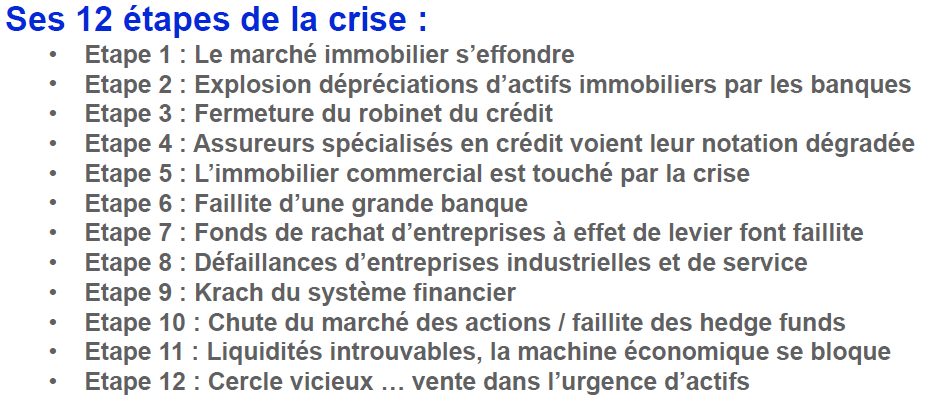
\includegraphics[scale=0.4]{7}
\end{center}

\subsection{Mais beaucoup rassuraient}
Même les organismes publics de contrôlent ne se doutaientt pas que la crise était possible. Une étude du FDIC \footnote{Federal Deposit Insurance Corporation : Institution publique américaine chargée d'assurer les consommateurs en cas de faillite d'une institution bancaire ou financière.} à l'été 2006 constate qu'il y a un développement rapide des produits non traditionnels ainsi que leur extension à des clients à profil risqué (les ménages à bas revenus) mais le plus important, l'augmentation de la valeur de l'immobilier qui limite les risques en cas de défaut. \\
On voit qu'en fait on a accumuler d'énormes risques en pensant que c'était sans risque.

\section{Faillite des grandes banques}
On a cru pendant longtemps qu'il était impossible qu'une grande banque fasse faillite parce que ça destabiliserai le système économique du pays. Aux USA, des petites et moyennes banques ont fait faillite mais on été reprises par d'autres banques et les épargnants n'ont rien perdu grâce à l'intervention de l'Etat (ce sont les actionnaires qui perdaient). En Europe, c'est moins fréquent et on a une meilleure protection des épargnants. Par contre, dans des pays moins développés, c'est très fréquent et les ce n'est pas toujours sans conséquence pour les épargnants. 

\subsubsection{Faillite de Lehman Brothers}
C'était une des 10 plus grandes banques américaines. Mais ils ont réalisé des pertes considérables sur à cause des sub-primes (20 milliards de dollars) et comme précédemment, les épargnants retirent leur argent et les autres banques refusent de prêter. \\
Une réunions des grandes banques américaines a été organisé sous la tutelle des autorités fédérales mais aucune banque ne veut reprendre Lehman sans une aide fédérale massive. Les autorités américaines refusent car l'aide est trop importante. Ce qui a conduit à la faillite de la banque. 

\section{La belle histoire de Fortis}
Une étape importante dans leur histoire a été l'acquisition d'ABN-AMRO. Celle-ci était un groupe financier hollandais diversié (banque et assurance) dont l'action en bourse évolue moins bien que les autres banques européennes. Les actionnaires sont donc mécontents (pas assez rentable) et mettent le management sous pression pour qu'ils vendent l'entreprise (on peut gagner beaucoup d'argent). La première offre de 61 milliards \$ vient de la banque anglaise Barclays. \\
C'est la que Merill Lynch propose une idée. C'était de diviser l'entreprise entre 3 investisseurs et chacun prendrait la part qui l'intéresse afin de rentabiliser les parts le plus rapidement possible. A l'époque tout le monde y croyait et on se doutait pas du risque des sub-primes. (exhubérance irrationnelle). Il suffisait donc de proposé plus que Barclays. 71 milliards \$ a été proposé par les 3 banques : Royal Banque of Scotland, Fortis et Santander. En Août 2007, les conquérants l'emportent. 

\section{Fortis et la finance mondiale}
Afin de comprendre la raison de cet achat par Fortis, regardons un peu l'histoire de cette banque qui est reprise sur les deux figures ci-dessous.\\
\begin{minipage}{0.55\textwidth}
	\begin{flushleft}
		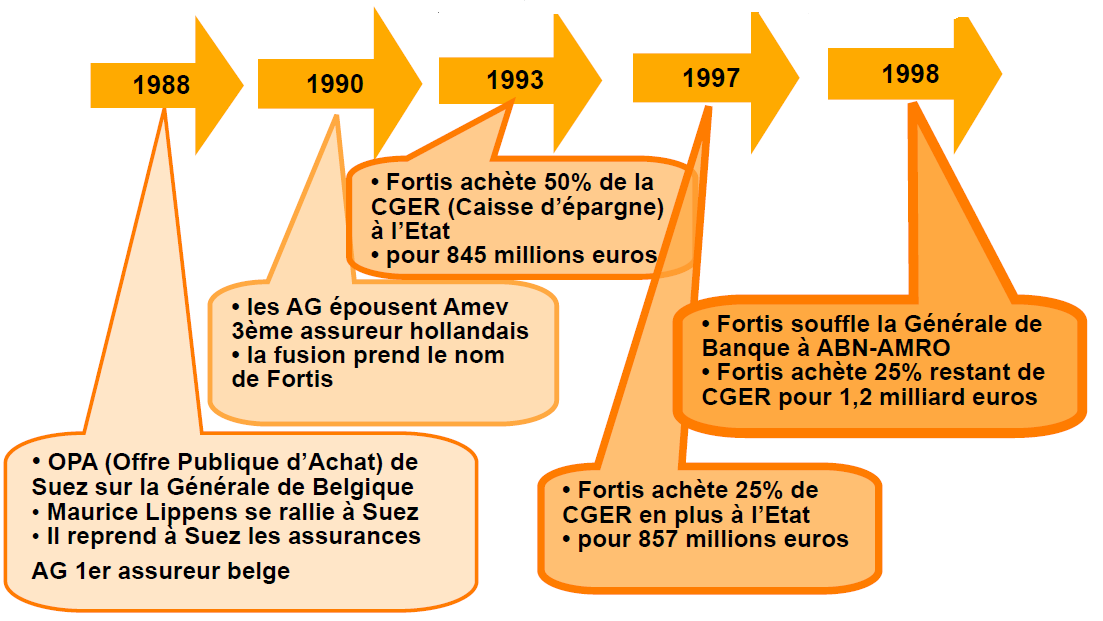
\includegraphics[scale=0.3]{8}
	\end{flushleft}
\end{minipage} 
\begin{minipage}{0.5\textwidth}
	\begin{flushright}
		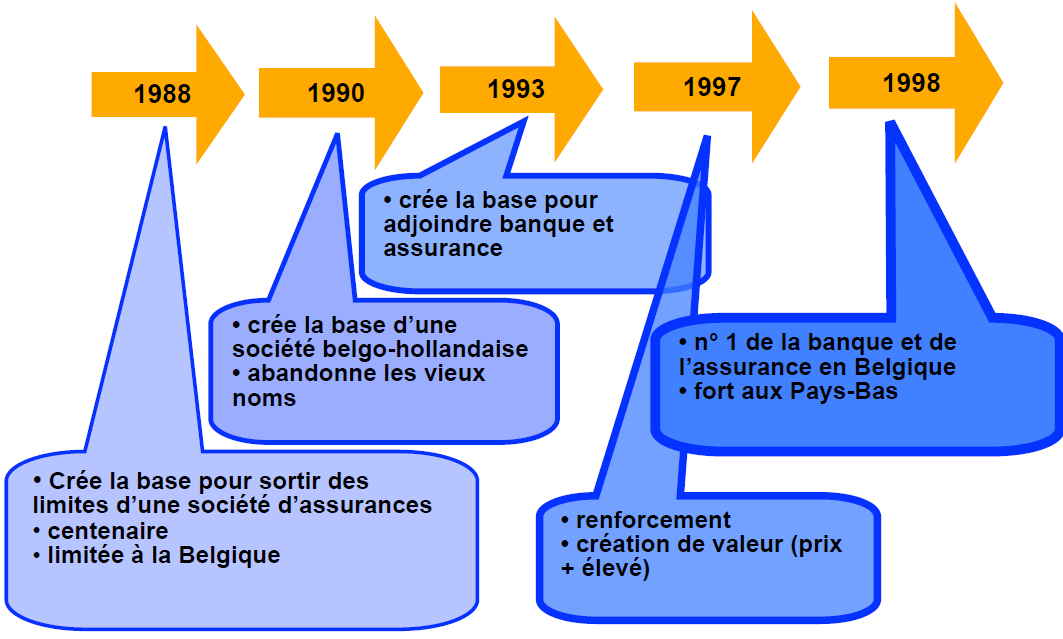
\includegraphics[scale=0.3]{9}
	\end{flushright}
\end{minipage} \\

Leurs motivations son repris en ces points : 
\begin{itemize}
	\item \textbf{Sortir des frontières} : il ne faut pas rester qu'en Belgique. Il faut s'étendre pour avoir de plus grand marchés $\rightarrow$ mondialisation.
	      
	\item \textbf{Acheter plutôt qu'être racheté} : si on est petit on se fera racheter par les plus grands. Donc il y a une certaine course à la taille. De plus, une même opération coûtent moins cher lorsqu'elle est reproduite en masse (comme dans l'industrie). Tout est informatisé donc le coût du système informatique reste inchangé quel que soit le nombre de clients également. Les produits est le même que ce soit en Belgique ou un autre pays. 
	      
	\item \textbf{La Banc-assurance} : l'assurance et la banque étant deux activités financières très proches, il y a un souhait de regroupement. Ceci permettrait non seulement de vendre ces deux produits aux mêmes guichets mais également d'utiliser les placements des assurances pour développer la banque.
	      
	\item \textbf{Grandir :} désir de passer d'une banque locale intégrée en une  banque international de marché. 
	      
	\item \textbf{Conservation du marché} : on veut attirer le plus de clients possible en transformant les entreprises poussiéreuse en quelque chose de rentable au maximum pour l'actionnaire.
\end{itemize}

Historiquement, Fortis désire passer d'une société privée conservatrice à une institution publique de crédit (à vérifier). Cependant, l'actionnaire classique considère toujours Fortis comme l'ancienne Générale de Belgique où les actionnaires sont des "bons pères de famille". Alors que les actionnaires internationnaux ont des exigences fote en matière de rentabilité et de prise de risque élevé. Donc, ça le motive également à aller chercher ailleurs. \\
Fortis devient l'une des 20 plus grandes banques mondiales et l'une des 10 plus granddes en Europe. \\
La banque grandit jusqu'à gérer des acifs d'une valeur de 410 milliards d'euros en 2007 et la valeur des produits générés a atteint 25 milliards d'euros (slide 9). 

\begin{wrapfigure}[8]{l}{8.5 cm}
	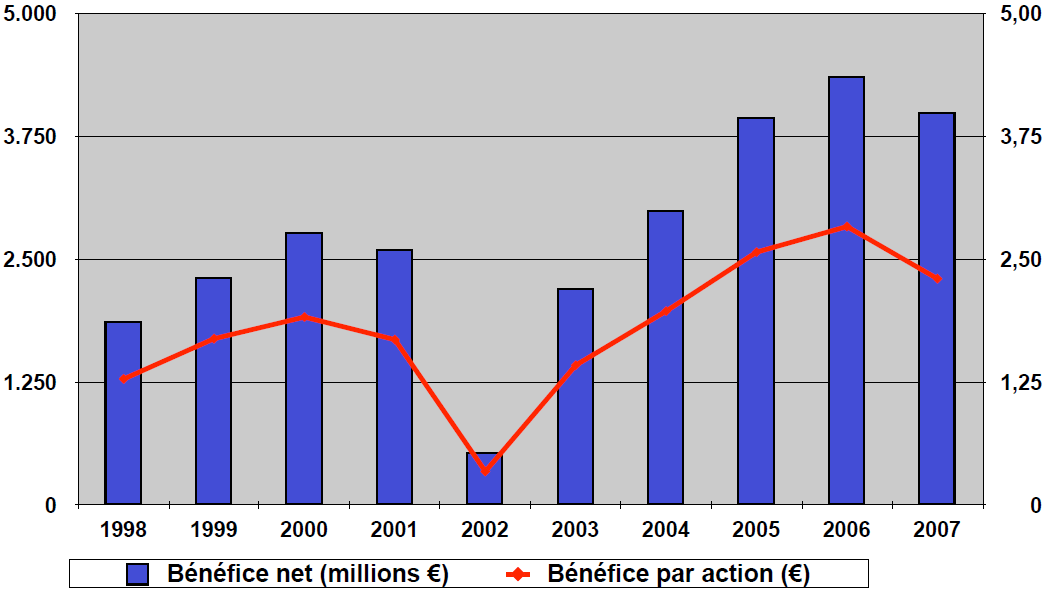
\includegraphics[scale=0.3]{10}
\end{wrapfigure}
\ \\ Cepedant, si on regarde le graphe ci-contre, on remarque qu'il existe une défaillance en 2002. Le bénéfice net et le bénéfice par action ont dégringolé malgré une évolution constante de la taille de la banque. Cette acciddent en 2002 a eu des conséquences diretes sur la valeur de l'action. 

\begin{wrapfigure}[10]{l}{8.5 cm}
	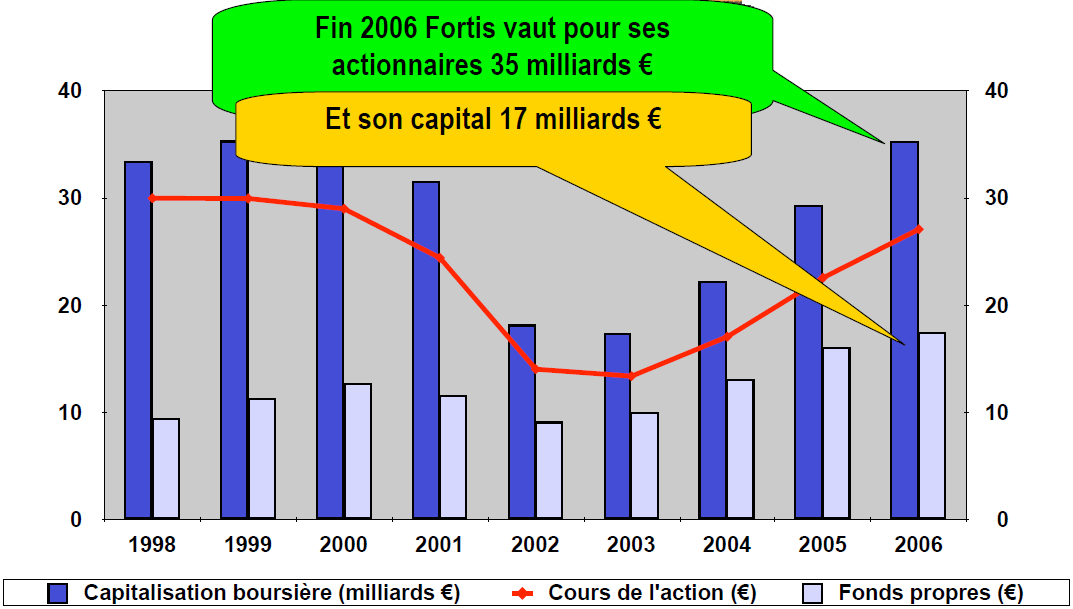
\includegraphics[scale=0.3]{11}
\end{wrapfigure}
\ \\ Quand on acquiert des actions, on espère qu'après un certain temps leur valeur augmentera. Cependant, pour Fortis, malgré la très bonne évolution, le cours de l'action est retombé entre 1998 et 2006. Fortis ne vaut en 2006, pour ces actionnaires, que ce qu'elle valait aproximativement en 1998 (35 milliards). Bien sûr, les actionnaires ne sont pas content. 

\section{ABN-AMRO, facteurs peu logiques}
Revenons à cette acquisition et montrons les facteurs pas très logiques. 
\begin{itemize}
	\item Si on refait l'état des lieux, Fortis vaut 35 milliards en bourse, son capital s'élève à 17 milliards et l'acquisition est de 24 milliards d'euros. C'est donc fou de se lancer dans une telle affaire! Mais elle est devenu n\degres 1 au Benelux : première banque, première assurance avec un Benelux qui compte 28 millions d'habitants dont le revenu fait partie des plus élevé. Elle est aussi l'une des 10 premières banques au monde pour les actifs en gestion \footnote{Les sommes confiées à la banque} mais aussi pour la gestion de fortune. 
	      
	\item Fortis expliquait vouloir s'étendre hors du Benelux. Or, là c'est tout le contraire qui se passe.
	      
	\item La commision européenne va exiger des cessions (vendre une partie de ce qu'on acquiert) pour éviter que Fortis ne soit trop dominant sur le marché du Benelux. De plus, il y a un risque à la revente parce que les délais de payement sont courts (pour l'acquisition).
	      
	\item Intégrer une grande banque sera difficile en raison des rivalité Fortis >< ABN-AMRO, des rivalités culturelles et les risques opérationnels importants (intégration technique). La rivalité entre les deux banques a commencé lorsque ABN-AMRO voulait acquérir la Générale de banque mais que Fortis l'a emporté. Mais aussi parce que le CEO de Fortis \footnote{Jean-Paul Votron} a été le n\degres 2 de ABN-AMRO dans le temps et a toujours voulu devenir n\degres 1.
\end{itemize}
On peut donc penser qu'il y a certains facteur émotionnels dans l'acquisition. 

\section{Acquisition d'ABN-AMRO}
Il faut décaisser au total 24 milliards d'euros. Les actionnaires de Fortis doivent fournir 13.5 milliards (confiance des actionnaires), 5 milliards seront empruntés aux marchés (confiance des autres banques) et on va devoir revendre 5.5 milliards à cause de la cession de la commission européenne. Il va donc faloir trouver des acquéreurs au bon prix. De plus, il faut que tout se passe bien. Donc il ne faut pas d'accident au sein de l'entreprise, ni dans les marchés. \\

Les prises de décisions se passent comme suit : 
\begin{enumerate}
	\item \textbf{Etude du projet} (début 2007) : par l'équipe de management et quelques administrateurs-clé. 
	      
	\item \textbf{Décision formelle d'y aller} (avril 2007) : par le conseil d'administration. 
	      
	\item \textbf{Décision de financement}(août 2007) : par l'Assemblée Générale Extraordinaire des actionnnaires.
	      
	\item \textbf{Assemblée Générale} (avril 2008) : C'est la que commence la dégringolade! "Décharge" (confiance) à tous les administrateurs et renouvellement de ceux-ci, dont Lippens et Votron (CEO).  
	      
	\item \textbf{Augmentation de capital d'urgence} (26 juin 2008) : décidé par 3 administrateurs sur un total de 13!!
\end{enumerate}

Afin de mieux comprendre la décision d'acquisition au sein de l'entreprise, un résumé du cadre professionelle dans une banque est disponible à la page suivante. 

\begin{center}
	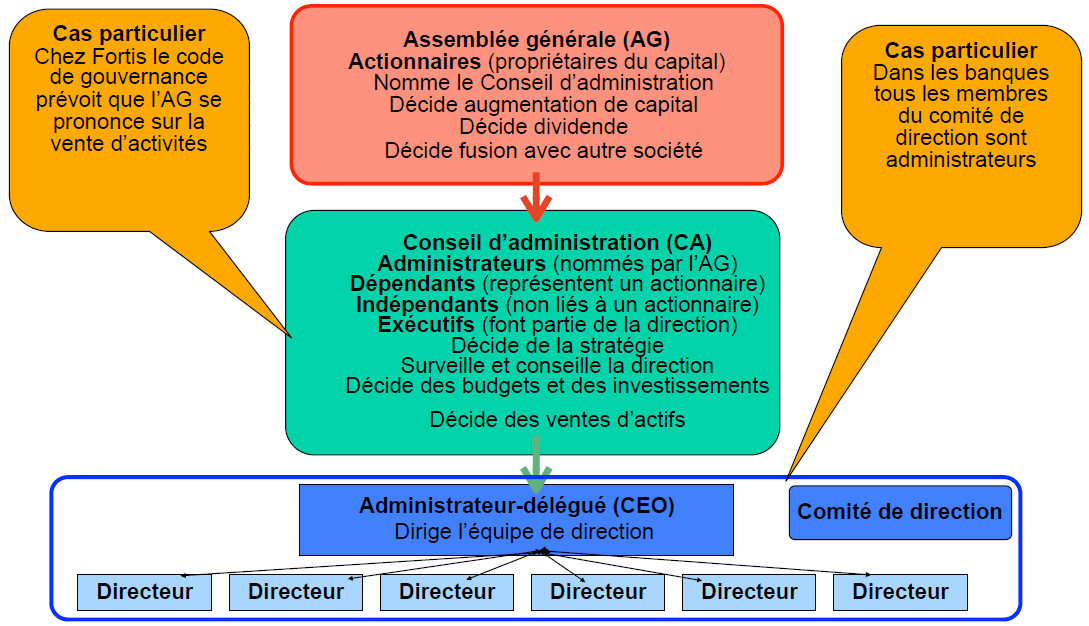
\includegraphics[scale=0.4]{12}
\end{center}

Voici maintenant un résumé de tous les événements qui se sont déroulé durant la chute de la valeur de l'action de Fortis. Comme on peut le constater, la chute va de pair avec la crise aux Etats-Unis. 

\begin{center}
	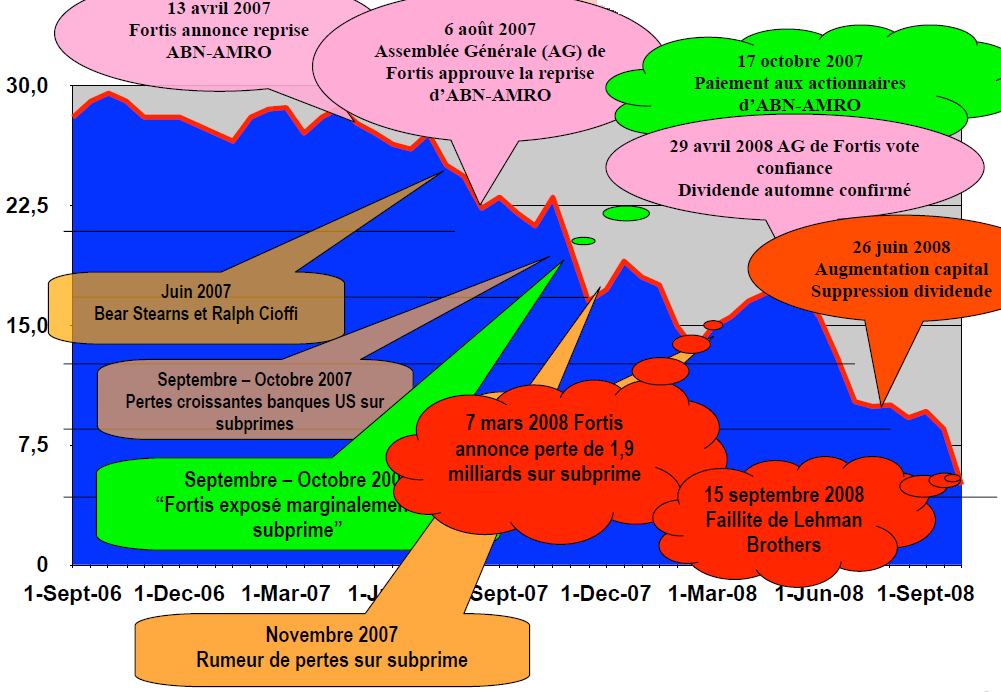
\includegraphics[scale=0.45]{13}
\end{center}

Durant cette fameuse chute, on a également une perte progressive de la confiance accordée à la banque. Les différentes raisons sont : 

\begin{itemize}
	\item \textbf{Augmentations successives de capital :} Même phénomène que pour Lehman Brothers, la valeur de l'action perd de sa valeur (-33\% en 9 mois!). Ceci mène à une perte de confiance des actionnaires.
	      
	\item \textbf{Information tardive sur les subprimes :} On joue avec les actionnaires car on leur annonce 4 mois plus tard qu'il y a une perte conséquente à cause des subprimes! On peut voir sur le graphe du dessus que les pertes surviennent vers septembre - novembre 2007 mais que l'annonce passe le 7 mars 2008. 
	      
	\item \textbf{Instabilité des dirigeants :} Départ du directeur financier et du CEO alors qu'ils venaient d'être nommés pour 4 ans. 
\end{itemize}

A partir de septembre 2008, les particuliers commencent à retirer leur dépôt mais le plus important, c'est que les grandes entreprises également les retirent. On a une perte considérable de cash. Après ça, les difficultés dans l'interbancaires croissent. "Le prédateur est devenu proie". \\
Fortis est particulièrement touché par la faillite de Lehman Brothers parce qu'elle avait vendu massivement des produits de cette banque. A partir du 25 septembre, les liquidité ne suffisent plus \footnote{Les besoins sont estimés à 40 milliards d'euro pour le 29 septembre.} et donc c'est la fin de la route, les Etats doivent intervenir. \\
La Belgique, les Pays-Bas et le Luxembourg augmentent le capital des banques Fortis (Bel,NL,Lux) et deviennent propriétaires à 50\% de ces banques. \\
Même cela ne suffit pas! On lègue totalement Fortis NL et ABN-AMRO à l'Etat hollandais, on vend les 50\% restants de Fortis Belgium à l'Etat Belge et l'Etat revend 75\% de cette dernière à BNP Paribas.
	%%%%%%%%%%%%%%%%%%%%%%%
%%      Lecon 3      %%
%%%%%%%%%%%%%%%%%%%%%%%

\chapter{Récession : de la crise de la finance vers celle des Etats}
\section{Résumé jusqu'ici}
Si on doit faire le résumé des 2 premiers chapitres : 
\begin{itemize}
	\item \textbf{La finance a radicalement changé en 20 ans} : Crédits risqués et endettements des ménages, innovations financière et effet de levier, course à la rentabilité, fragentation du métier bancaire.
	      
	\item \textbf{Exhubérance irrationnelle :} On est en pleine euphérie irrationnelle c'est à dire qu'on est dans nos dreams on pense que tout ira bien et on fait des hypothèses très optimistes.
	      
	\item \textbf{Puis perte de confiance :} des épargnants, des actionnaires, des autres banques et du personnel. 
	      
	\item \textbf{Faillite de grandes banques :} on ne pensait pas que c'était possible. 
	      
	\item \textbf{On se tourne vers les Etats :} plus rien ne va donc les risques et profits privés deviennent publics au détriment de l'endettement des Etats.  
\end{itemize}

\section{Mesure en économie - frêt maritime}
On a par exemple le \textbf{Dry Baltic Index} (BDI) originaire de Virginia and Baltick Coffeehouse. \footnote{Londres - Financial District (1744)} Le fonctionnement est simple, les courtiers en fret maritime récoltent tous les jours et dans le monde entier les prix du frêt et on calcul un indice global qui sera publié.\\
Cette indicateur à ses inconvénients et montrons les dans le cadre du transport maritime. Le BDI fluctue très fort en cas de déséquilibre offre-demande. En effet, la demande peut varier du jour au lendemain mais l'offre ne sait pas suivre (les bateaux sont là). Ceci entraine de grands changements de prix avec la demande. Elle ne permet pas de prévoir l'économie mais permet de voir les tendance du commerce mondial (de biens matériels). 

\begin{wrapfigure}[10]{l}{9cm}
	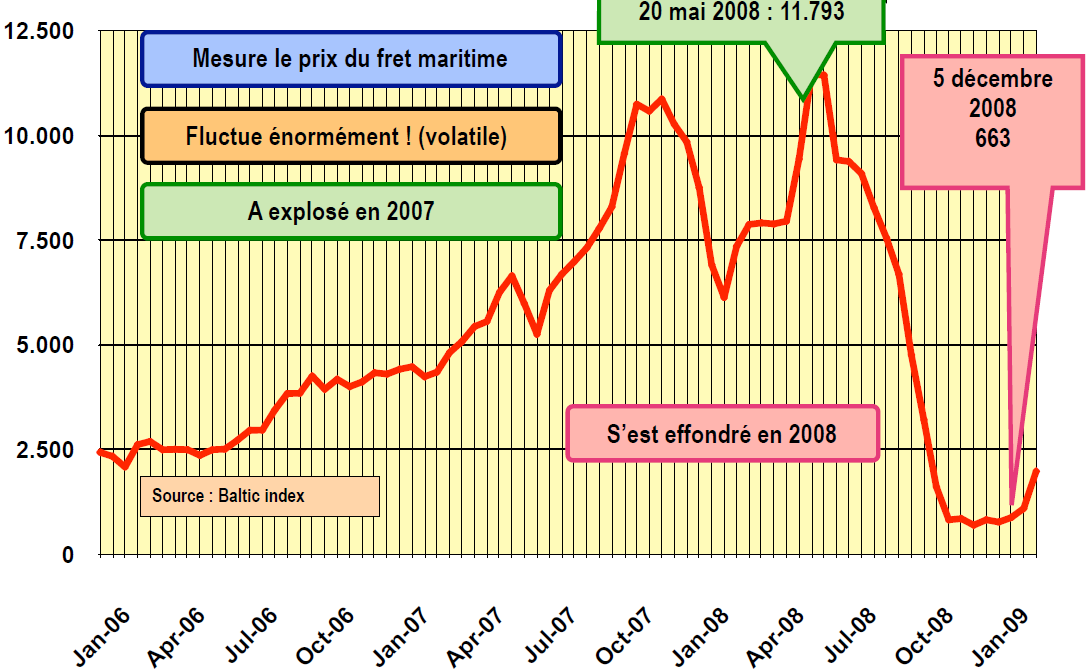
\includegraphics[scale=0.3]{14}
\end{wrapfigure}  
Regardons maintenant le BDI pour le frêt maritime (à gauche). Comme on peut le voir, les prix se sont effondrés en 2008. Comment est-ce qu'on adapte l'offre dans ce cas là ? Parce que si le marché monte trop, ça attire les investisseurs et donc ça favorise l'achat de nouveaux bateaux. C'est ce qui se passe dans notre graphe et c'est très mauvais pour la chute subite. \\
Solutions : A long terme, on peut reporter ou annuler les commandes aux chantiers navals ou même envoyer les vieux bateaux à la casse. A moyen terme, on doit mettre les navires à l'ancre (ne travaillent pas) mais beaucoup d'entreprises font faillite. A court terme, on diminue la vitesse des bateaux pour réduire la capacité et on économise ainsi du fuel. 

\section{La chaîne de la crise}
\begin{wrapfigure}[8]{l}{9cm}
	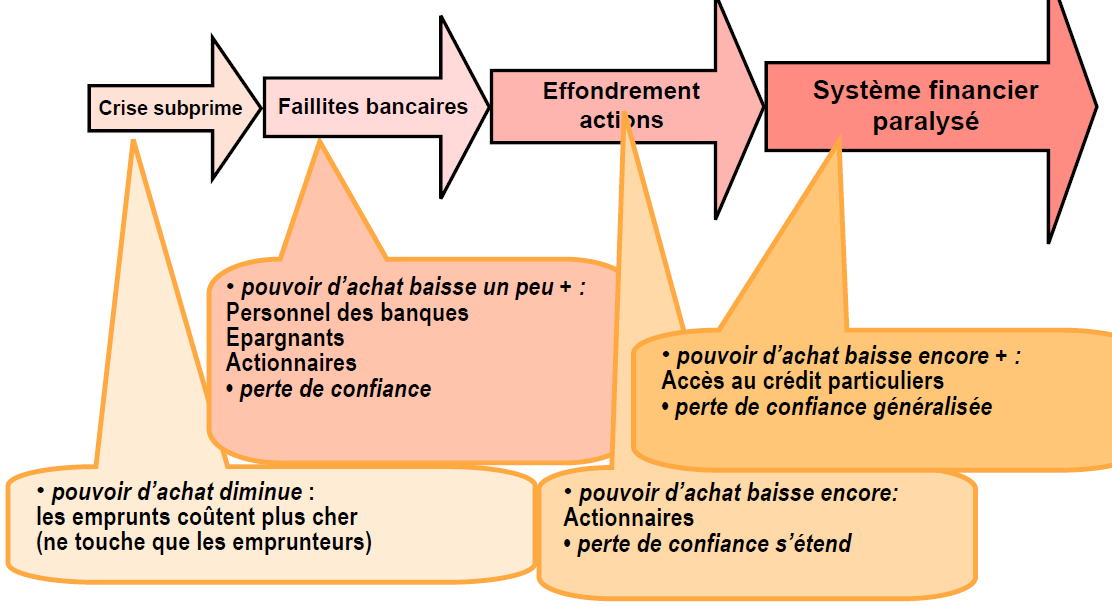
\includegraphics[scale=0.3]{15}
\end{wrapfigure}
Comme on l'a vu dans les chapitres précédents, tout à commencé par la finance. Un résumé en ligne du temps est présenté à la figure ci-dessous. Nous allons voir maintenant comment la crise de la finance s'est manifesté dans les autres secteurs, notamment dans l'industrie automobile.\\\\

\subsection{Crise dans l'industrie}

\begin{wrapfigure}[12]{l}{9cm}
	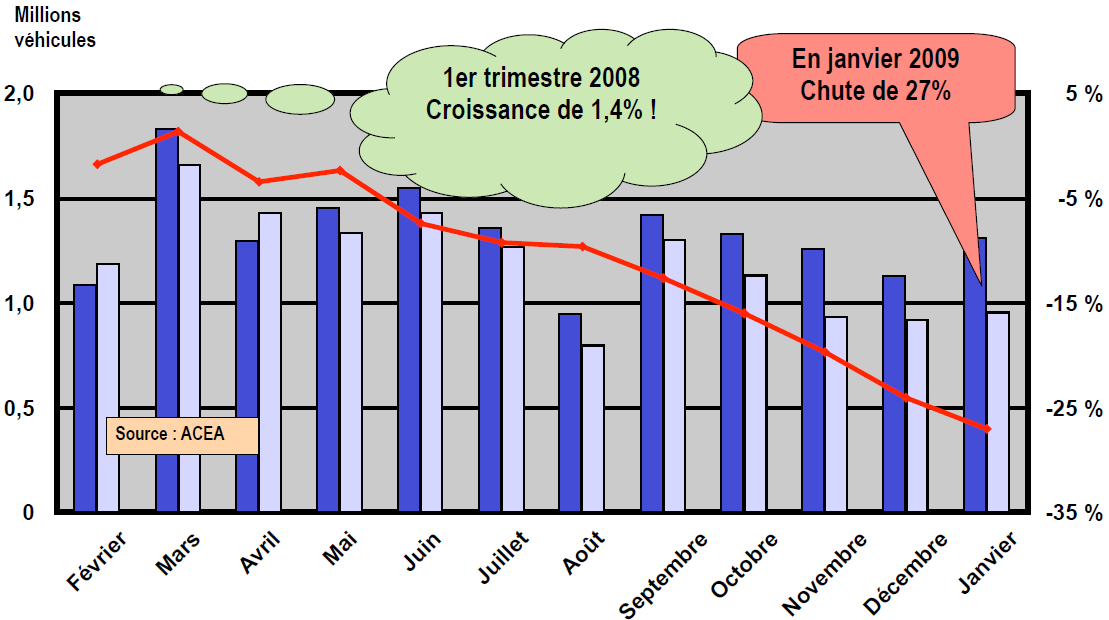
\includegraphics[scale=0.3]{16}
\end{wrapfigure}
\ \\ Comme on peut le voir sur la figue ci-contre, le secteur automobile se porte très mal. On voit que la vente d'automobile en 2008 et 2009 est bien plus faible qu'en 2007 et qu'elle s'accentue au fil des mois. De plus, tous les pays ne sont pas touché de la même manière. Par exemple, en janvier 2009, on observe une chute de -27\% réparti en : Espagne -41.6\% , UK -30.9\% , Belgique -16.1\% et la France -7.9\% .\\
Bien sûr ce n'est pas le seul secteur touché. Tous les types de bien et tous les fabricants sont touchés mais pas de la même façon : pneus Michelin -15.0\% , GSM -5.0\% mais Nokia -15.0\% , ... On a donc une véritable chute de la demande de biens durables. 

\begin{wrapfigure}[11]{l}{9cm}
	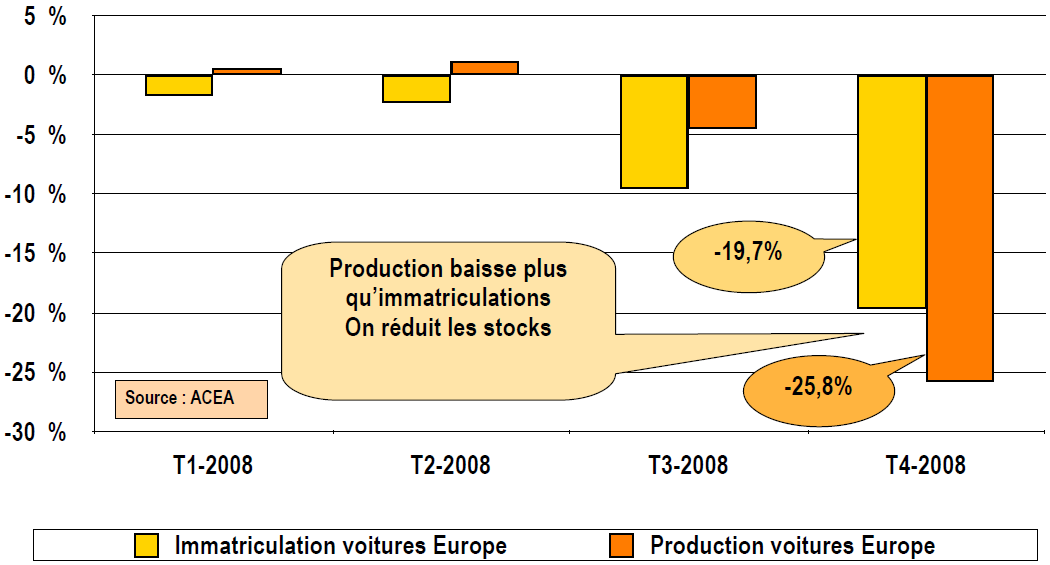
\includegraphics[scale=0.3]{17}
\end{wrapfigure}
Quelle est la réaction des entreprises ? Elles vont évidemment essayer de se protéger et vont réduire leur production de telle manière à arriver en fin 2008 à baisser la production beaucoup plus par rapport à la baisse des immatriculations. Ceci a pour conséquences des licenciements, des chômages techniques et une cessession d'embauche qui limite encore plus le pouvoir d'achat. De plus, les entreprises diminue fortement leur investissements dans la construction de nouveaux lieux de travail et donc la nous sommes dans un cercle vicieux puisque le même processus que dans le secteur automobile se manifestera (demande $\searrow$ production $\searrow$ frêt $\searrow$ emploi $\searrow$ ).

\begin{wrapfigure}[11]{l}{9cm}
	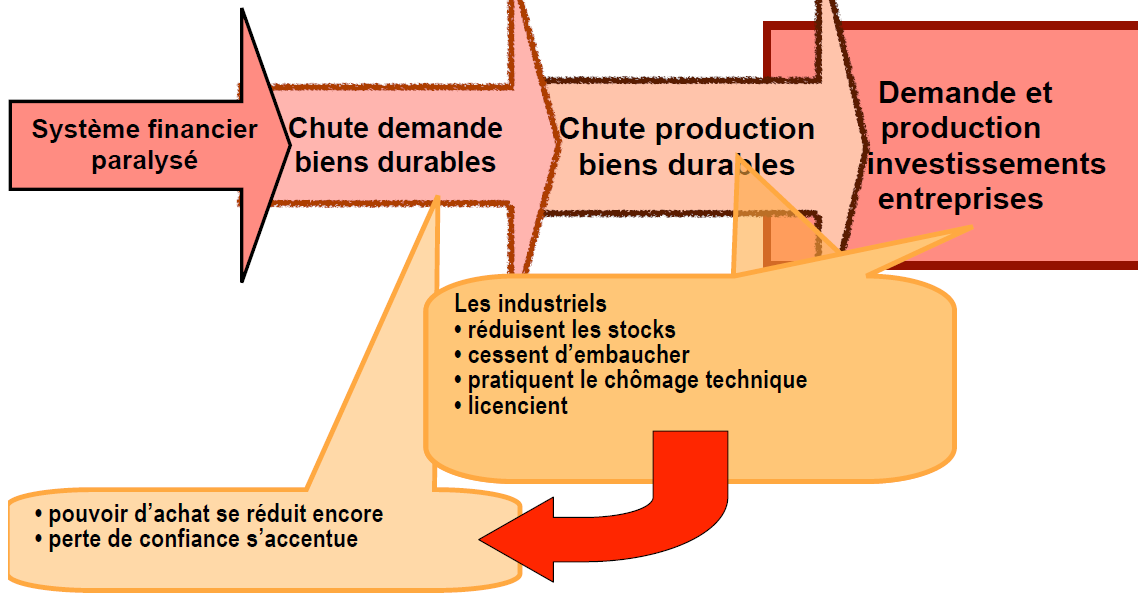
\includegraphics[scale=0.3]{18}
\end{wrapfigure}
La crise que nous observons commence à se manifester dans tous les pays. On peut voir que l'Allemagne, dont l'économie est fortement influencé par l'automobile et les machines, possède la plus grosse baisse de PIB. Cependant, cette crise commence à toucher le monde entier. En effet, les pays d'Asie qui exportent énormément vers l'Europe et les USA vont voir celles-ci chuter. Par exemple, Taiwan perd 42\% de ses exportations, l'Inde 22\%, etc. (graphique slide 4). La crise mène donc à une dépression économique mondiale ! 
\begin{center}
	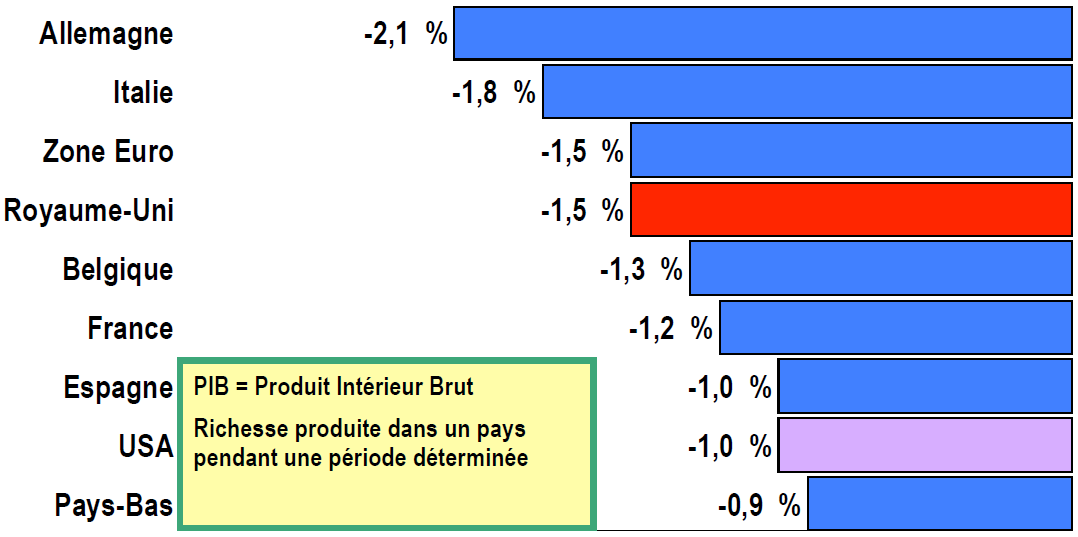
\includegraphics[scale=0.4]{19}
\end{center} 
\subsection{Crise des matières premières}
La matière première la plus importante est l'acier puisque c'est le composant de base pour les biens durables et d'investissement. Si on regarde le premier graphique, en 2006, on a une explosion de la demande notamment grâce à la croissance excellente de la Chine et l'Inde. Seulement, avec tout le processus de crise, la demande chute jusque 25\% par rapport à l'année précédente. C'est la plus grosse chute après la WW2. Ceci se généralise à toute forme de matière première. Le prix du baril de pétrole (fort indicateur pour l'économie mondiale) s'effondre en 2008 ! On voit de nouveau ce phénomène de forte croissance juste avant la chute (v. 2$^{ème}$ graphique).
\\\\
\begin{minipage}{0.55\textwidth}
	\begin{flushleft}
		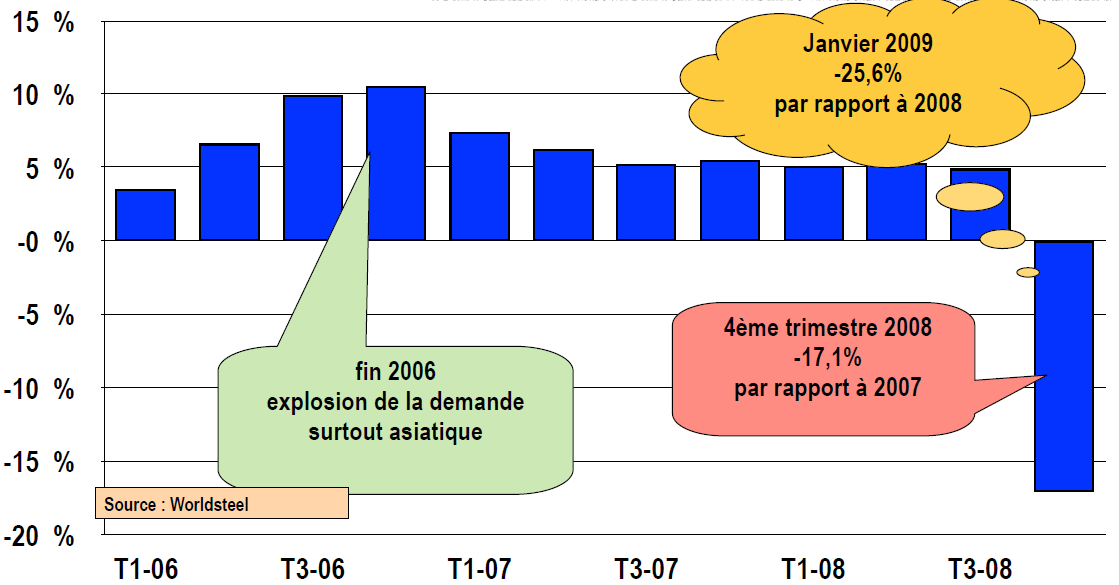
\includegraphics[scale=0.28]{20}
	\end{flushleft}
\end{minipage}
\begin{minipage}{0.5\textwidth}
	\begin{flushright}
		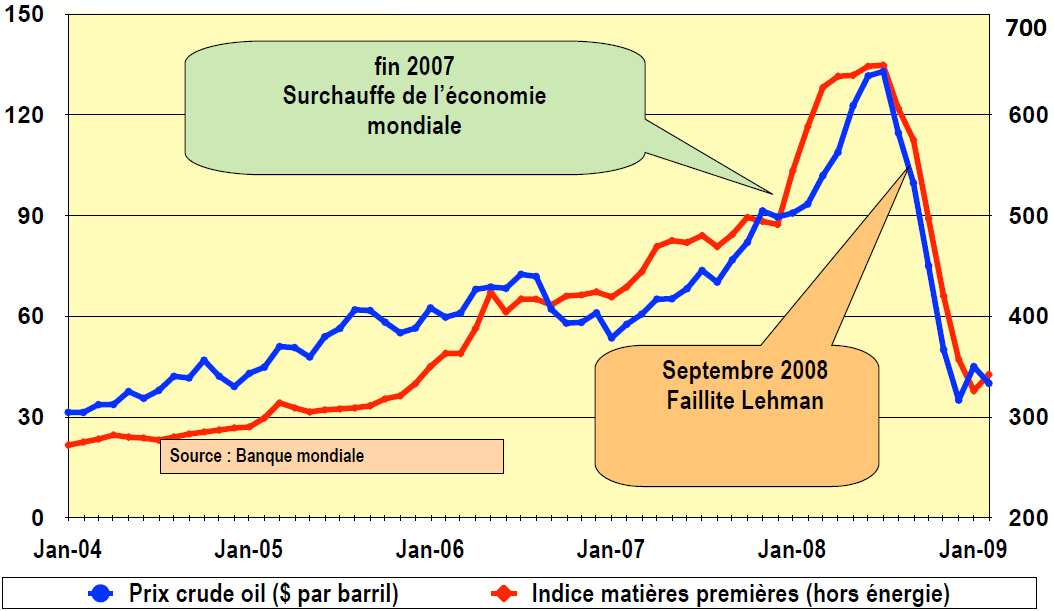
\includegraphics[scale=0.3]{21}
	\end{flushright}
\end{minipage}
\\\\
La mondialisation fait en sorte que la crise prend une plus forte empleur et devient de plus en plus conséquent puisque le cercle viscieux s'aggrave et n'est pas prêt de s'arrêter puisque les consommateurs perdent toujours leur confiance. 

\begin{center}
	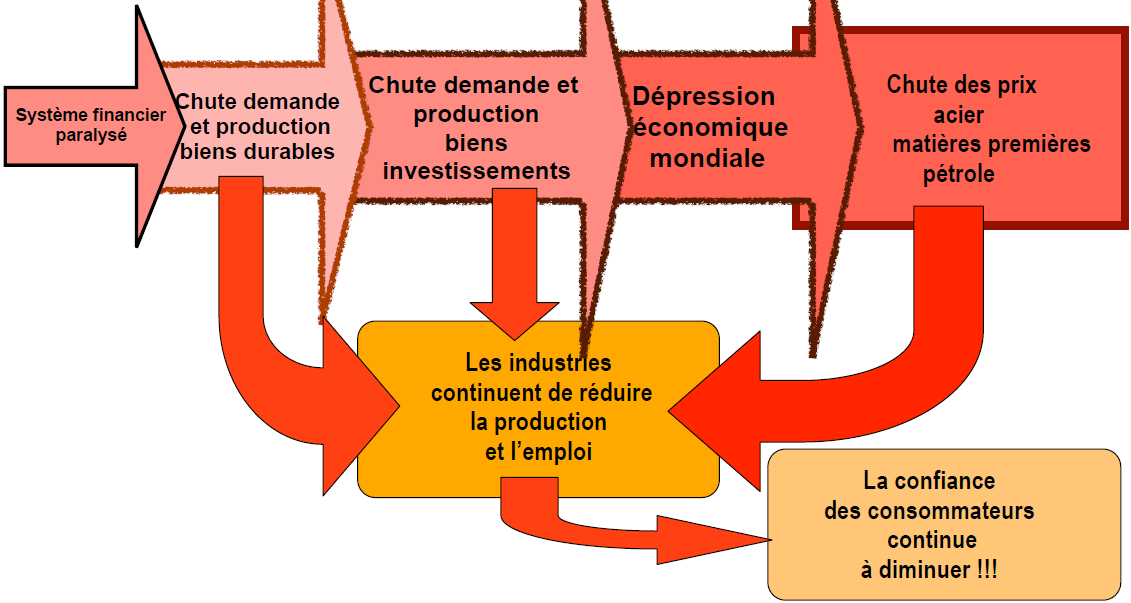
\includegraphics[scale=0.4]{22}
\end{center}

\section{Actions de sauvetage}
\subsection{Dégradation des prévisions}
\begin{wrapfigure}[13]{l}{9cm}
	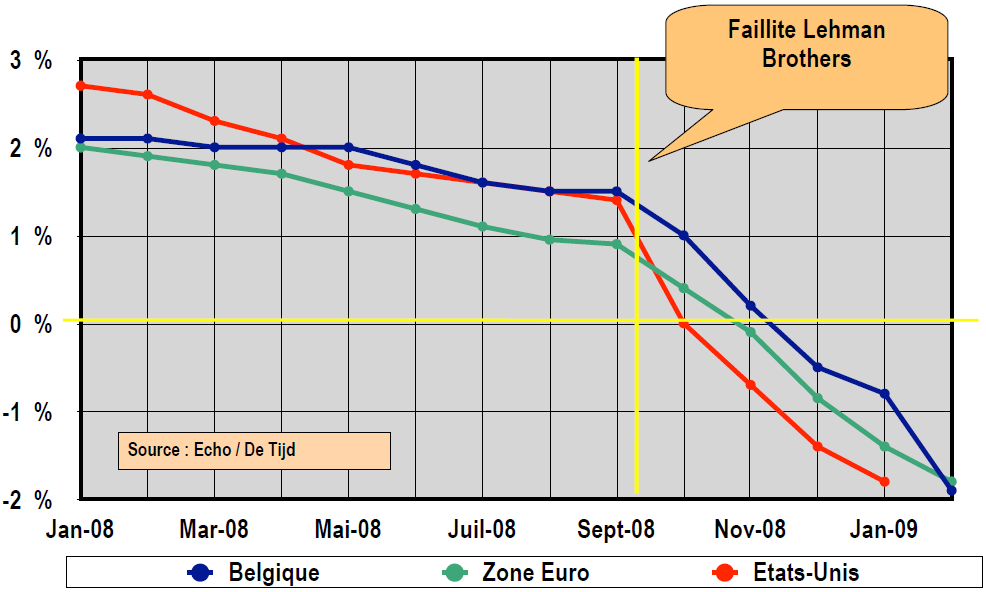
\includegraphics[scale=0.35]{23}
\end{wrapfigure}
Le rêve de tout économiste est de pouvoir prédir le cours de la finance. C'est très compliqué parceq que des événements se produisent tous les jours et influe cette dernière. Cependant, certains expert essaye d'anticiper les évolutions futures d'après les modèles qu'ils établissent. Ca permet à tout le monde de se faire une idée avant d'investir. Voici ci-dessous une prévision pour le PIB de certains états. On peut voir que la \textbf{faillite de Lehman Brothers} a provoqué un tournant dans les prévisions et les économistes ne sont plus très optimistes pour la suite. En effet, la crise fait perdre confiance à tout le monde, la demande et la production de biens durables chute, les investissements aussi, le pouvoir d'achat baisse à cause des pertes d'emploi et reprend la boucle du début. Comment éviter une crise comme en 1929-30 ?

\subsection{La crise économique évitée}
A partir de février 2009 jusqu'en fin 2010, les Etats ont mené des actions rigoureuses et coordonnées. De plus, plus le temps avance, plus on a de nouveaux besoin. Donc on peut accéder à de nouveaux marchés en innovant. L'immobilier reprend petit à petit et on essaye de désendetter les ménages et leur permettre une épargne. Tout ça permet de briser la chaine de récession et les premiers signes de reprise apparaissent. C'est l'Asie qui sort en premier de ce cercle viscieux et a déjà presque oublié la récession. Cependant, on a éviter la crise au détriment des Etats qui se sont endettés lourdement. Nous allons tout droit vers la crise des Etats !

\subsection{Etat des lieux et évolution après dépression}
\begin{wrapfigure}[8]{l}{8cm}
	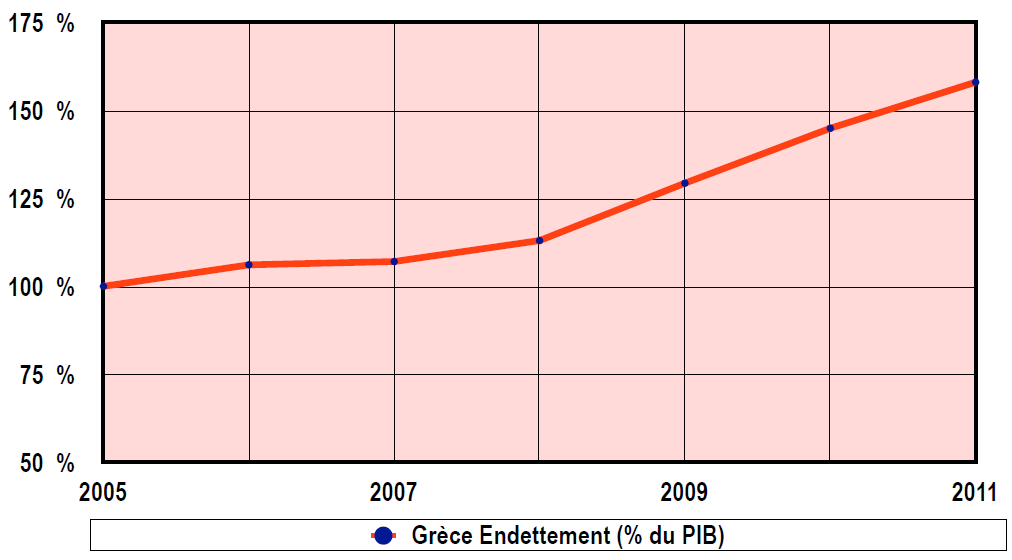
\includegraphics[scale=0.28]{24}
\end{wrapfigure}
\ \\ Comme on l'a cité juste au point précédent, les Etats s'endettent lourdement. Si on regarde l'évolution jusqu'en 2011 de la dette greque, on peut confirmer la crise de cet Etat, alors qu'on pensait que les Etat ne pouvvait pas faire faillite. La Grèce a divisé les opignons en deux (Grexit or No Grexit). 

\begin{wrapfigure}[6]{l}{8cm}
	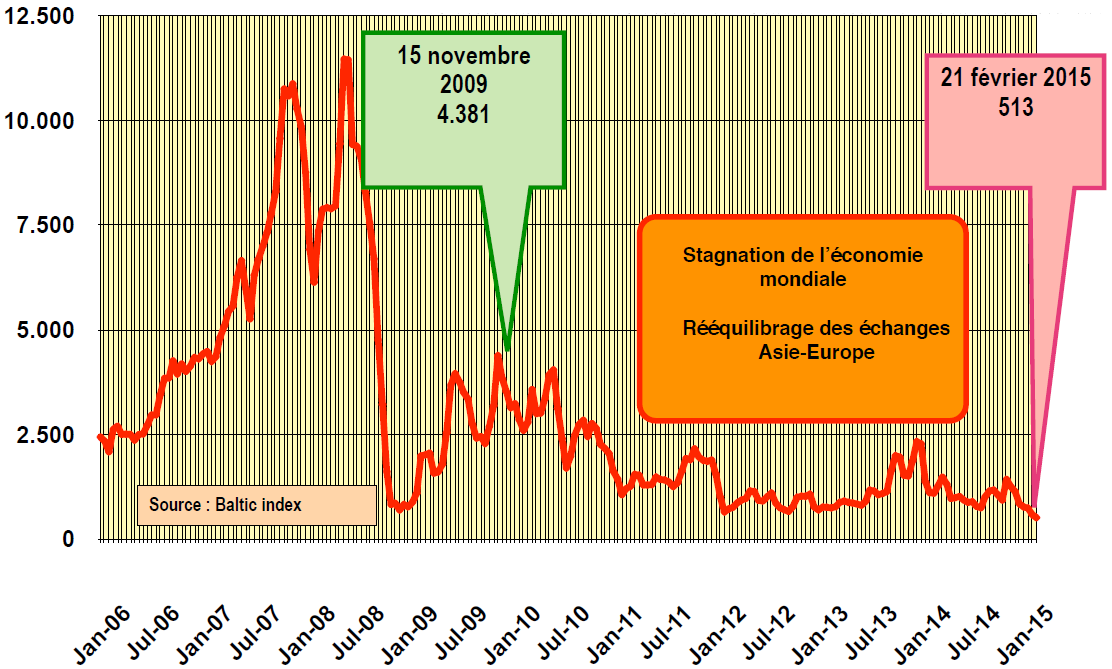
\includegraphics[scale=0.26]{25}
\end{wrapfigure}
\ \\ Aussi, on a peut-être évité une crise, mais l'économie mondiale ne s'en est pas remis après ces événement. La Dry Baltic Index, nous montre une stagnation du prix du frêt et donc un équilibrage des échanges inter-Etats. \\\\

\begin{wrapfigure}[9]{l}{9cm}
	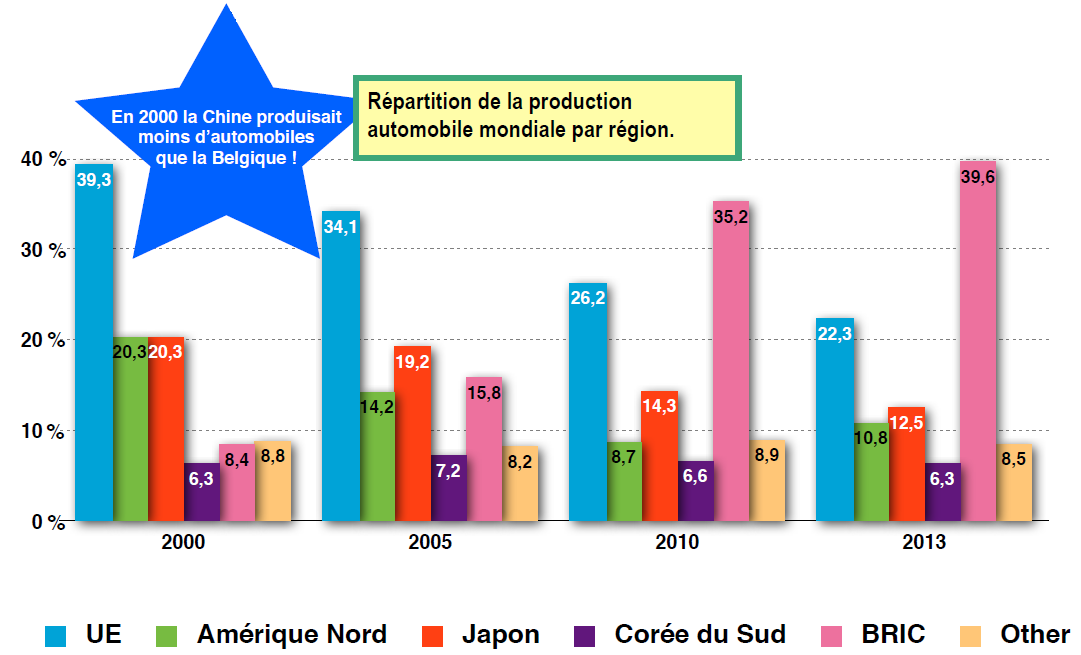
\includegraphics[scale=0.32]{26}
\end{wrapfigure}
\noindent Par contre, on observe sur ce graphique que l'Asie s'est très bien tiré de l'affaire et a provoqué un changement du centre de gravité de l'économie mondiale. Les grandes puissances auparavant qui étaient les Etats-Unis et certains pays d'Europe, laisse la place à la \textbf{BRIC} (Brésil, Russie, Inde, Chine) auquel on peut inclure l'Afrique du Sud.  
	%%%%%%%%%%%%%%%%%%%%%%%
%%      Lecon 4      %%
%%%%%%%%%%%%%%%%%%%%%%%

\chapter{Action, crise des Etats et crise de l'Euro}
\section{Rappel du cercle vicieux}
Voici en 3 images, le résumé de la situation expliquée dans les chapitres précédents. Je trouve que les schémas sont bien faits et ne nécéssite pas d'explication supplémentaires.\\
 
\begin{minipage}{0.5\textwidth}
	\begin{flushleft}
		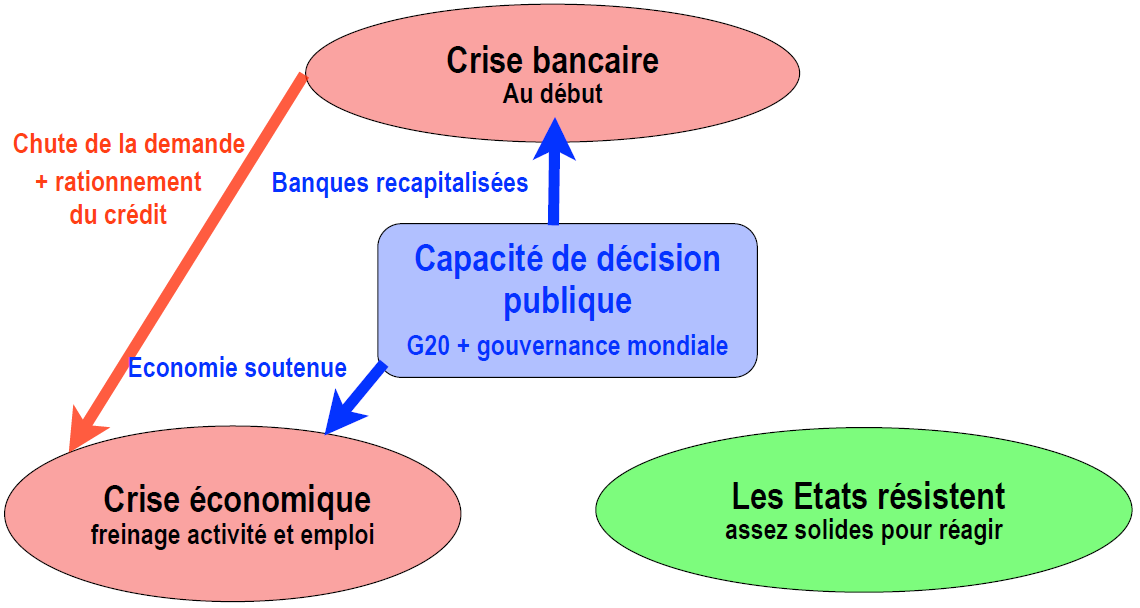
\includegraphics[scale=0.26]{27}
	\end{flushleft}
\end{minipage}
\begin{minipage}{0.5\textwidth}
	\begin{center}
		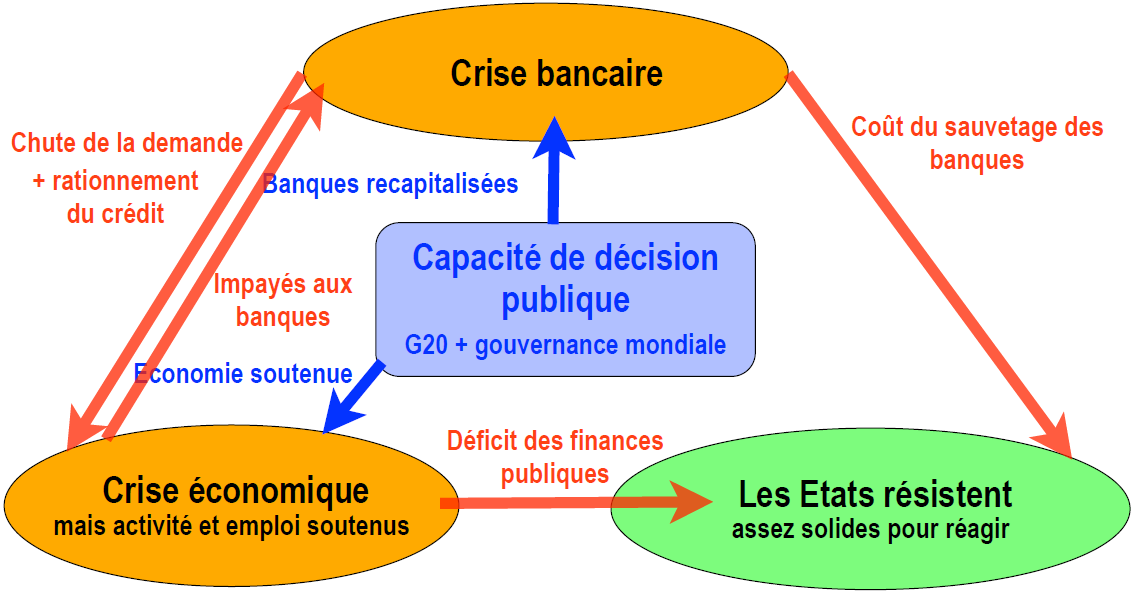
\includegraphics[scale=0.26]{28}
	\end{center}
\end{minipage}
\ \\
\begin{center}
	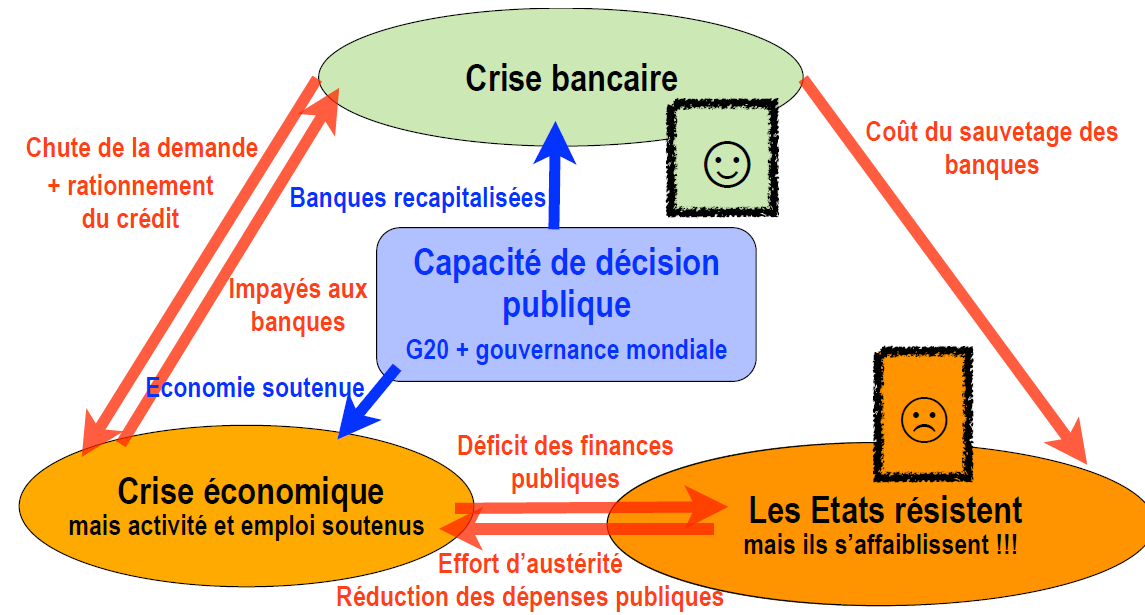
\includegraphics[scale=0.3]{29}
\end{center}

\section{Construction de l'Europe}
\subsection{Le début}

\begin{itemize}
	\item \textbf{1948 - 1952, les fondements intellectuels :} \\ 
	      On vient de sortir d'une grande guerre et il faut rebâtir l'Europe. Schuman, Adenauer et Monnet commencent à réfléchir à une union.
	      	
	\item \textbf{1952, Communauté Européenne du Charbon et de l'Acier :} \\
	      Il faut relancer l'industrie européenne. 6 pays décident de créer une alliance économique et non militaire : All, Fr, It et Benelux. On élargira la coopération à Euratom (nucléaire) par la suite.
	      	
	\item \textbf{1957-1958, Traité de Rome :} \\
	      La CECA s'élargie à la Communauté Economique Européenne qui devient donc un marché commun (suppression progressive des frontière) et dont l'éxécutif est la Commission Européenne. La coopération de l'Allemagne et de la France crée un axe très solide. 
\end{itemize}

\subsection{Un long chemin}
On a du parcourir un long chemin, avant d'en arriver à l'union d'aujourd'hui. Dans les grandes lignes, on a eu :

\begin{itemize}
	\item \textbf{De nombreux échecs :} \\
	      En 1953, la création d'une Communauté Européenne de Défense a échoué. En 1965 et 1967, la France pose son véto à l'entrée de la Grande Bretagne dans l'union. Et en 1970, les nombreuses tentatives de monnaie unique ont échouées.
	      	
	\item \textbf{Des élargissements successifs :} \\
	      Aux 6 pays créateurs se sont ajoutés, le UK, le Dannemark et l'Irlande en 1973, la Grèce qui était passé à la démocratie en 1981 et l'Espagne et le Portugal qui sont également des démocraties mais qui sont également de grands concurrents agricoles pour les pays membres, en 1986.
	      	
	\item \textbf{Des approfondissements financiers :} \\
	      On créa, en 1979, le Système monétaire Européen (SME) qui se chargeait des fluctuations des différentes monnaies présentes dans l'union pour avoir des devises assez liées. 
	      	
	\item \textbf{Mais aussi démocratiques :} \\
	      On éli les membres pour le Parlement européen pour la première fois en 1979 et on signe le Traité de Schengen de libre circulation en 1985.
\end{itemize}

\subsection{Le grand bond en avant}
Cette union a eu énormement de succès, dont :

\begin{itemize}
	\item \textbf{1989, chute du mur de Berlin :} \\
	      Celle-ci partageait l'Allemagne en deux et seul la partie ouest faisait partie de l'union. L'intégration de cette partie directement posait problème aux Français puisque l'Allemagne allait gagné en voix. Cependant, les Français acceptait l'intégration de la partie Est si l'Allemagne était d'accord d'adopter l'Euro. 
	      	
	\item \textbf{1992, Traité de Maastricht :} \\
	      On signe ici une union politique qui donne à l'Union Européennne des compétences étatiques et on forge une union monétaire, l'Euro. 
	      	
	\item \textbf{Les Etats abandonnent des compétences souveraines :} \\
	      Comme émettre la monnaie, la politique judiciaire, de police, pénale et la politique de sécurité extérieure (ex : instabilité en ex-Yugoslavie).
	      
	\item \textbf{1995, Suède, Autriche, Finlande :} \\
	      L'intégration de ces pays a été rendu possible par la fin du communisme. 
	      	
	\item \textbf{2004, ex pays de l'est et Méditerrannée :} \\
	      On intègre la Slovénie, Slovaquie, Tchéquie, Pologne, Hongrie, les Pays Baltes, Malte et Chypre.
	      	
	\item \textbf{2007, Roumanie et Bulgarie.}
	      	
	\item \textbf{2013, Croatie.}
	      	
	\item \textbf{Pour le futur :}
	      L'Europe attire toujours la Serbie, Montenegro, Macédoine, Albanie et la Turquie.
\end{itemize}

\section{L'Union Monétaire et l'Euro}
\subsection{Le difficile traîté de Maastricht}
Quelles étaient les éxigences des pays face à une union monétaire ? Ils voulaient avoir une évolution économique parallèle avec, notamment, la même croissance, inflation, coût salarial et la même compétitivité sur le marché, mais aussi un contrôle sur les déficits.\\
On voulait également avoir des économies qui ne réagissent pas trop différemment aux chocs économiques pour garder ce parallélisme. \\
Ce n'est pas tout. On voulait avoir des mécanismes aptes à remédier aux écarts entre les pays, comme prendre des décisions d'états coordonnées, contrôler l'évolution des salaires et des prix, mais aussi avoir une bonne politique de migration des travailleurs et des capitaux. 

\subsection{Les risques}
Cependant, il y avait certains problèmes. Tout d'abord, les pays du centre étaient bien plus industrialisés que les pays de la périphérie, ce qui provoquait une divergence économique. De plus, la cohérence politique sur certains points est incertaine. Malgrés cela, il fallait adopter cette monnaie commune en raison des taux de change flottants qui conduisent à de l'instabilité, la mondialisation, la libralisation de la circulation des capitaux (risqué car fait fluctué la monnaie) et la volonté des acteurs principaux en Europe. \\
Cependant, on a signé un \textbf{pacte de stabilité} qui limite le déficit public et impose la supervision de la Commission Européenne. On veut aller plus loin dans la coopération en autorisant les réformes structurelles dans la compétitivité, pensions et l'intégration politique.

\subsection{Naissance et élargissements de l'Euro}
Malgré toutes les difficultés, 11 Etats choisissent l'adoption de la monnaie commune. En 1999,, les marchés financiers adoptent donc l'euro (marché des changes, la bourse, la dette publique, les trésoreries des entreprises). Et dès le 1er jannvier 2002, on utilise la nouvelle monnaie. \\
Il y a eu des élargissement par la suite. Entrent dans l'euro, la Grèce en 2001, la Slovénie, Chypre et Malte, Slovaquie, Estonie et en 2014 la Lituanie. On décide que tous les nouveaux pays adhérant à l'UE doivent adopter l'euro quand les conditions sont remplies. 

\section{Cohésion à l'épreuve}

\begin{wrapfigure}[7]{l}{8cm}
	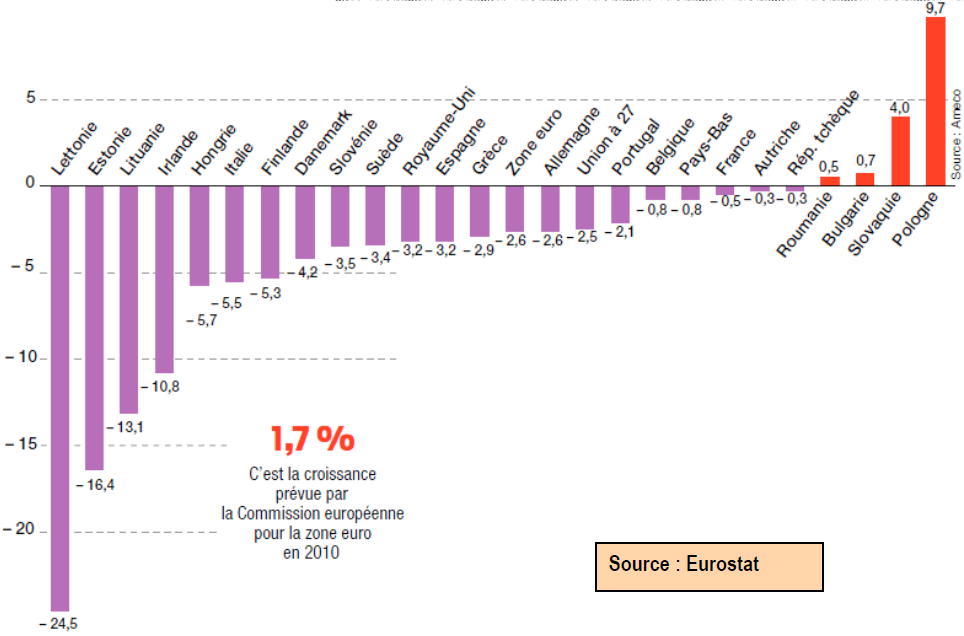
\includegraphics[scale=0.3]{30}
\end{wrapfigure}
\noindent Par contre, ça ne va pas très bien dans la zone euro. On avait dit qu'on ne voulait pas de disparité au niveau de la croissance des Etats mais c'est tout le contraire qui se passe ici. Les "grands pays" subissent une décroissance de leur PIB alors que les pays les plus à l'est tire profit de la nouvelle alliance. \\\\\\

\begin{wrapfigure}[7]{l}{8cm}
	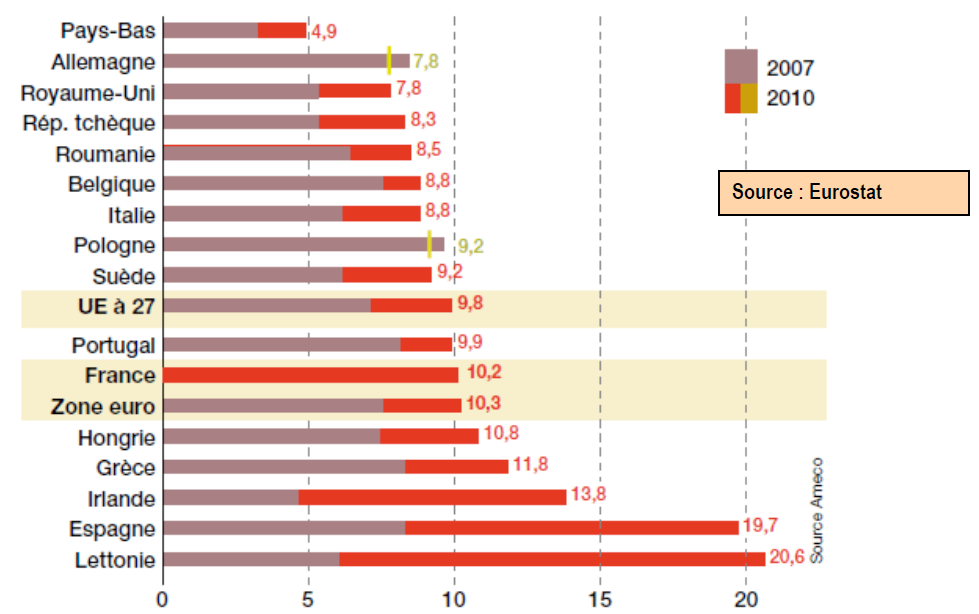
\includegraphics[scale=0.3]{31}
\end{wrapfigure}
\noindent Ceci est en grande partie dû à la forte montée du chômage au sein de la zone euro qui atteint les 20\% en Espagne et Lettonie. La Lettonie est d'ailleurs le pays le plus touché d'après le graphique précédent. De nouveau, les chiffres sont très différents d'un pays à l'autre. C'est le deuxième élément de divergence. \\\\\\

\begin{wrapfigure}[11]{l}{8.5cm}
	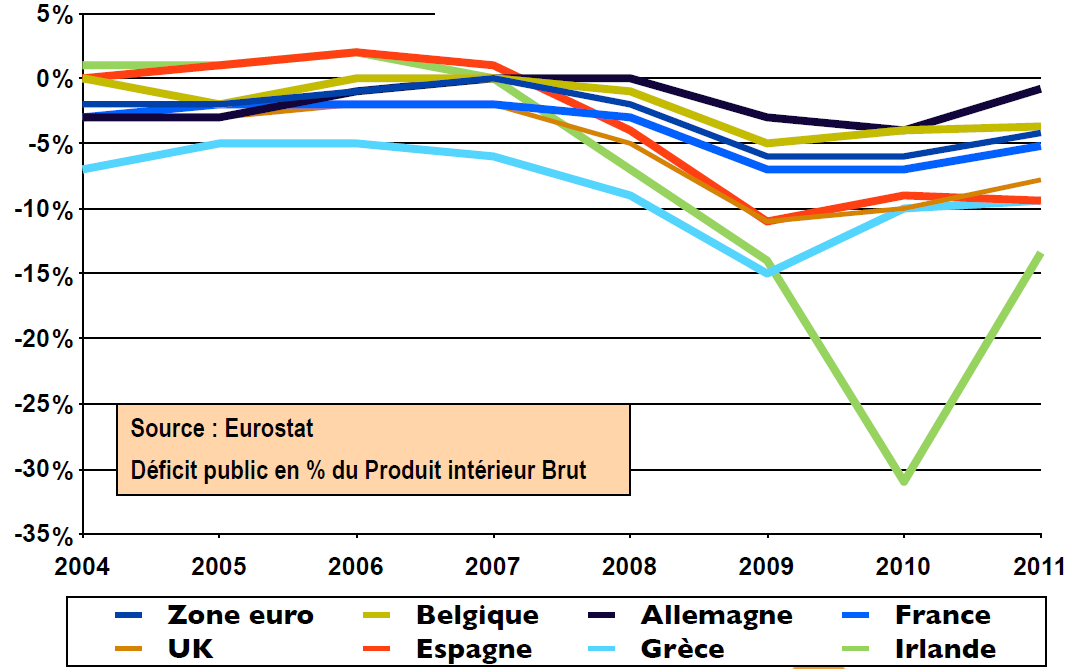
\includegraphics[scale=0.3]{32}
\end{wrapfigure}
\noindent Le troisième élément de divergence est la différence que l'on rencontre dans les déficits. En effet, selon le graphique, on peut voir un mouvement d'ensemble pour certains pays mais également d'autres pays comme l'Irlande qui ne suivent plus du tout la cohésion. Le déficit de l'Irlande atteint d'ailleurs les 25\% ce qui est un grand signe d'instabilité. \\\\\\\\

La très forte pression sur le budget des Etats (en raison de l'aide aux banques) va faire qu'à un moment, le budget ne supporte plus. Ceci fait monter l'austérité et influence l'économie globale qui se porte de plus en plus mal. Ceci met les Etats encore plus en difficulté  et sont forcés de couper certaines aides aux banques. Ceci mécontente les banques et instabilise totalement l'économie. Les Etats sont, dès lors, obligés de s'endetter.

\begin{wrapfigure}[11]{l}{9cm}
	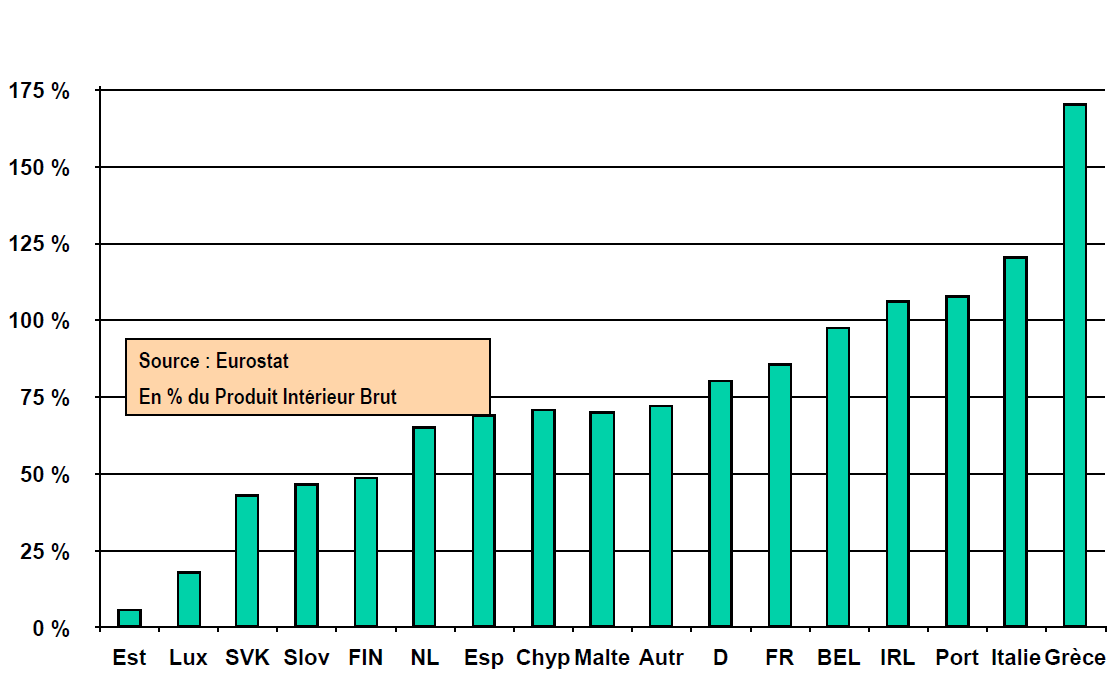
\includegraphics[scale=0.3]{36}
\end{wrapfigure}
\ \\ \\ La dernière et la plus importante des divergence s'observe au niveau des dettes publiques. Le graphe montre très bien ce phénomène et met en avant un problème majeur : la dette de la Grèce qui a atteint les 175\% de sont PIB. Beaucoup d'autres pays sont au dessus des 100\% de dette, ce qui traduit également une inefficacité de l'union.

\section{Situation de la Grèce}
\subsection{L'entrée dans l'euro}
Les critères à valider pour entrer dans l'euro sont : avoir un déficit des finances public inférieur à 3\% du PIB et la dette public doit être inférieur à 6\% ou doit diminuer chaque année. Jusqu'en 1994, la dette de la Grèce reste supérieur à 10\% donc ne sait pas entrer dans l'euro. Mais elle annonce en 1999 que son déficit est en dessous des 3\% donc peut entrer dans la zone euro en 2000. Elle doit maintenant pouvoir maintenanir ces 3\% et pour ça, elle va faire preuve de "créativité" économique et va utiliser, dès 2001, des instruments financiers qui permettent de cacher une partie de la dette. \\
Cependant, à partir de 2002, les doutes commencent à se réveiller car il y a un changement à partir de 2000 sur les données de la Grèce. On a des difficultés à voir clair. Les doutes commencent aussi pour d'autres pays comme l'Italie et le Portugal. 

\subsection{Première alerte en 2005}
Eurostat refuse de valider les chiffres grecs ! Ceci survient juste avant les élections mais le nouveau gouvernement va entreprendre des audits approndie afin de résoudre cette énigme. Celui-ci révèle des déficits bien plus élevés que ceux déclarer !\\
De ce fait, la Comission Européenne ouvre les procédure d'infraction contre la Grèce car le déficit est supérieur à 3\%. Mais pas seulement en Grèce. En Italie, Allemagne, France et Portugal aussi. Néanmoins, la Grèce réussi quand même à ramener son déficit à 2.6\% en 2006 (contre 5.5\% en 2005) donc tout va bien.

\begin{wrapfigure}[10]{l}{9cm}
	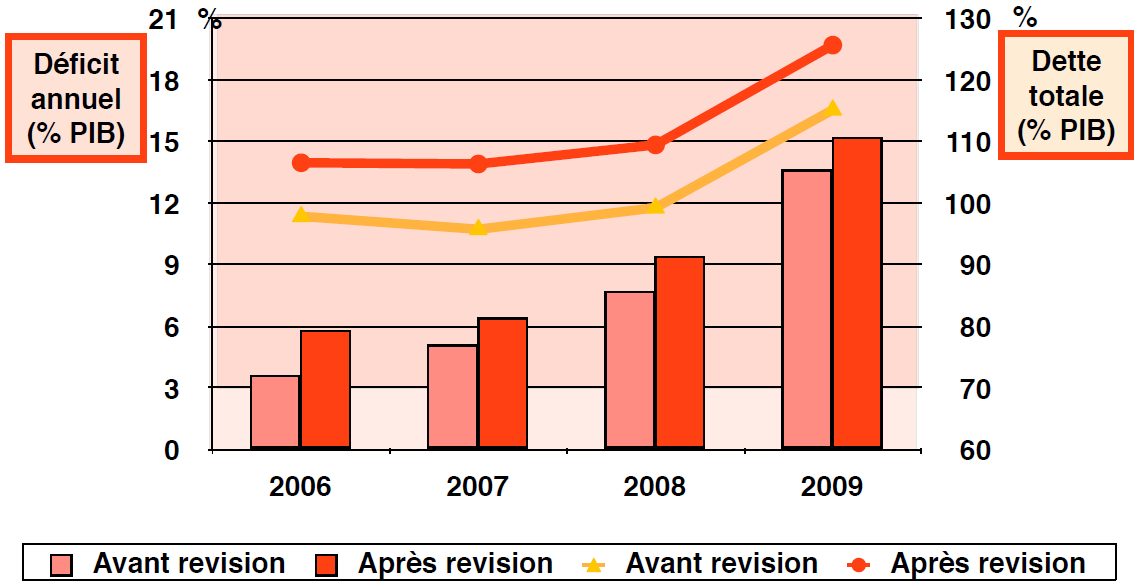
\includegraphics[scale=0.3]{37}
\end{wrapfigure}
\ \\\\On décide en 2009 de faire une révision des chiffres. C'est ici que la vérité est découverte. Les chiffres sont bien plus élevés que ce que les Grecs ont déclarés. Si on ajoute à cela l'épisode de la crise en 2007, la situation s'aggrave et la confiance accordée au pays est fortement perturbée. Les conséquences sont :

\begin{enumerate}
	\item La « notation »\footnote{C'est l'apréciation donnée (note de confiance) par une agence à un pays. Cela permet de connaître les pays à risque et ceux où il est bon d'investir.} de la dette grecque est dégradée de A à BBB+ le 16 décembre 2009
	      
	\item Les capitaux fuient le pays vers d'autres où ils seront en sécurité.
	      	
	\item Les taux d’intérêt grecs augmentent.
\end{enumerate}   

\begin{wrapfigure}[9]{l}{9cm}
	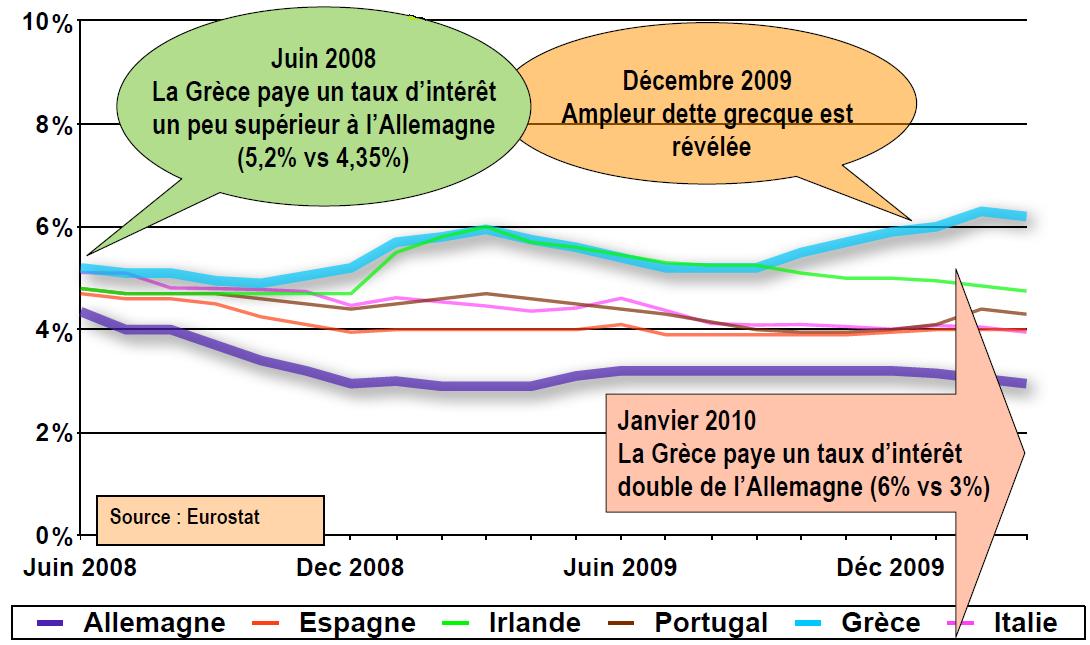
\includegraphics[scale=0.3]{38}
\end{wrapfigure}
\ \\ Une des conséquences majeures est que le taux d'intérêt reste assez élevé comparé aux autres pays. Ceci est en partie dû à la perte de confiance et la difficulté de remboursement des prêts. Il faut apporter un soutien rapidement pour remédier à cette situation. \\\\\\\\

\subsection{Plan de sauvetage}
Le gouvernement grec adopte un plan de réduction drastique du déficit (dépenses militaires, hopitaux, retraite, gel du nombre de fonctionnaire et baisse des salaires) et diminue ses dépenses de 52.0\% à 50.6\% du PIB de 2009 à 2010. \\
Le gouvernement relève les recettes du pays de 39,3\% à 41,9\% du PIB de 2009 à 2010 grâce à une réduction de la fraude fiscale, des taxes supplémentaires, impôts sur les entreprise et l'immobilier et hausse de la TVA.\\
Par ailleurs, l'Europe avait promis une aide financière. Mais la pression sur les marchés ne diminue pas ! Le 23 avril 2010, la Grèce demande l'aide du FMI et de l'EU.\\
L'EU appelle à la solidarité financière pour assurer la survie de l’euro. Pas seulement pour la Grèce mais aussi pour l’Espagne et le Portugal (voire l'Italie). On prépare des fonds de stabilisation de 750 Milliards d'euros dont 60 milliards empruntés par la Commission européenne, 440 milliards euros apportés par les Etats européens (Belgique : 15 puis de 27 milliards) et 250 milliards euros apportés par le FMI. On prête à la Grèce de 110 Milliards d'euros, soit 10.000 euros par grec ! Cependant la pression des marchés financiers ne va pas s’arrêter. Les gestionnaires de fonds continuent à quitter la Grèce et à investir dans les pays sûrs.

\subsection{Résultat du plan de sauvetage}
\begin{wrapfigure}[12]{l}{9cm}
	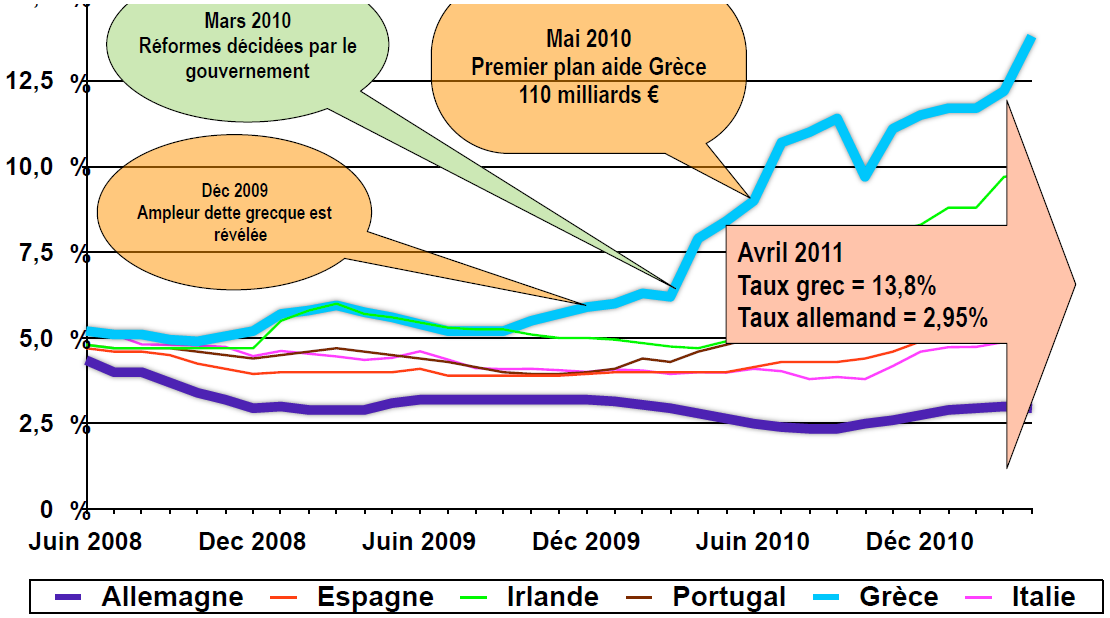
\includegraphics[scale=0.3]{39}
\end{wrapfigure}
\noindent On est dans une véritable crise de gouvernance. L'aide est tardive et le résultat est décevant. Comme on peut le constater, le taux d'intérêt de la dette de la Grèce ne cesse d'augmenter et est exhorbitante par rapport à celui de l'Allemagne. Pour ce qui est de l'évolution annuelle du PIB, elle décroche en 2009 et ne cesse de diminuer (-8.9\% en 2011). Pareil pour le PIB/habitants, elle descend de 63\% de celle des Belges à 50\% (diapos 10-13 pour les graphiques).\\
Nous sommes dans une impasse (mai 2011) parce que la Grèce n’est plus capable d’emprunter, la population grecque s'oppose progressivement à l‘austérité et donc on ne sait plus mettre en place des réformes fiscales structurelles. Petit à petit, les pays européens se divisent. Doit-on faire payer les emprunteurs seulement ou les prêteurs aussi ?\\
De juillet à Octobre 2011 ont lieu des négociations intenses. On décide d'accélérer l’intervention internationale de 110 milliards euros et d'abandonner une dette de 50 milliards (par les banques privées nationales et internationales). L’essentiel de la dette grecque est dorénavant détenu par les autres états. Malgré cela, le plan de réformes (austérité) doit être poursuivi.

\begin{wrapfigure}[13]{l}{9cm}
	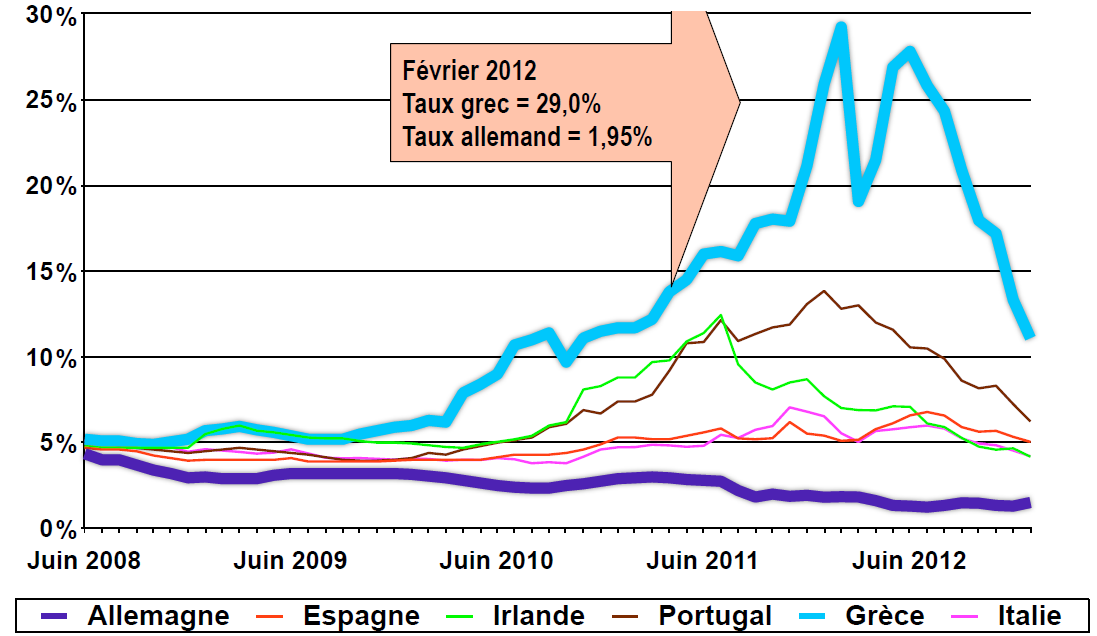
\includegraphics[scale=0.3]{40}
\end{wrapfigure}
\ \\ On voit que les grandes décisions prises en 2011 ont fortement contribué à la réduction du taux d'intérêt. Néanmoins, cela reste insuffisant et de nouvelles actions de solidarité doivent être mené en Grèce, Irlande, Portugalet Espagne. Mais les opignons publiques rejettent les plans d'austérité et entraine des conséquences potiques (montée du nationalisme, protectionnisme, repli sur soi, populisme anti-européen). On observe aussi la montée des extrêmes en Italie (élections de février 2013) et en Grèce (élections de janvier 2015). \\
D'autre part, la solidarité financière est rejetée par les opinions publiques des
pays « riches » (Allemagne, Finlande, Pays-Bas, et même France) ce qui provoque une faiblesse institutionnelle de l’Union européenne.

\subsection{Deux visions sur la crise greque}
Voici les deux slides qui reprennent assez bien les deux opignons. La première présente les causes et la deuxième, les solutions. 

\begin{center}
	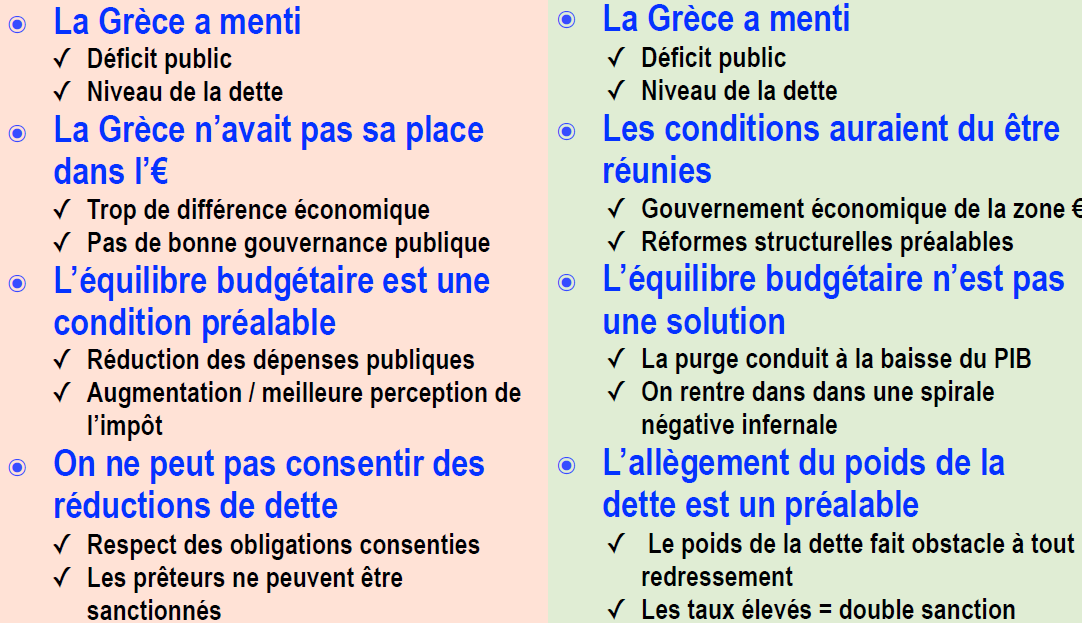
\includegraphics[scale=0.5]{41}
\end{center}

\begin{center}
	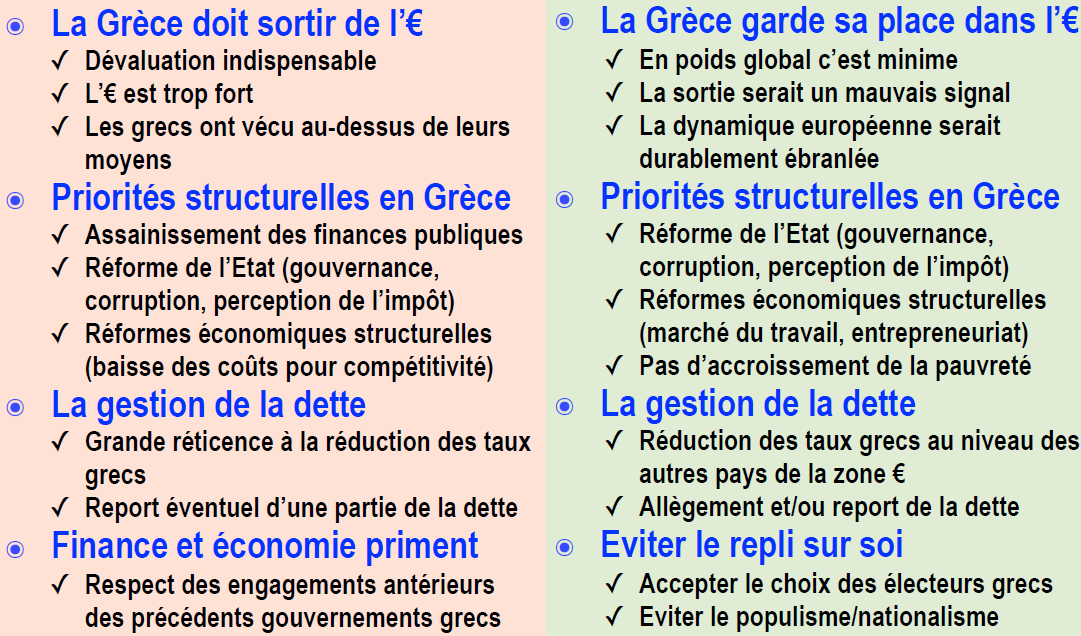
\includegraphics[scale=0.5]{42}
\end{center}
	%%%%%%%%%%%%%%%%%%%%%%%
%%      Lecon 5      %%
%%%%%%%%%%%%%%%%%%%%%%%

\chapter{Les leçons de la grande crise de 1929 :
similitudes et différences}

Avant de passer à la crise de 1929, on peut résumer les derniers cours dans leurs grandes lignes de la sorte : 

\begin{center}
	Innovation financière + exhubérance irrationnelle $\rightarrow$ faillite de grandes banques + perte de confiance (actionnaires, épargnants, etc.) $\rightarrow$ les Etats interviennent $\rightarrow$ économie réelle en difficulté $\rightarrow$ Etats endettés $\rightarrow$ entraîne l'Euro dans la tourmante.
\end{center} 

\section{Les crises dans l'histoire}
\subsection{Japon 1990}
Vers la fin des années '80, la bourse japonaise explose. La valeur des actions est haute et les taux d'intérêt sont assez bas (2.5\%). Cependant, en 1990, la première guerre du golf éclate. Ca entraine une chute de la demande (crise du pétrol) ainsi qu'une remontée des taux d'intéret à 4.5\%. Les emprunteurs sont alors en difficulté et des banques font faillites (on passe de 22 grandes banques à seulement 8), ce qui fait encore plus chuter la demande. On observe une croissance faible pendant 10 ans (1,6\% par an de 1990 à 2002 contre 3,3\% par an de 1980 à 1990) et l'indice boursier reste aussi bas qu'en 90 en 2009.

\subsection{USA 1987}
Les « savings \& loans » (caisses d’épargne) sont petites et mal gérées. De plus, une innovation financière risquée fait son apparition : les « junk bonds ». Ce sont des prêts risqués aux entreprises pour faire effet de levier, à taux d'intérêt élevé mais à déficiences fréquentes quand la conjoncture se dégrade. En 1989, a lieu la crise immobilière et financière. Les « savings \& loans » font faillites (leur nombre passe de 4000 à 1500) mais les banques qui ont investies en « junk bonds » aussi. Il faut donc l'intervention de l’Etat, la RTC (« Resolution Trust Company ») prête 150 milliards US\$ et la FDIC (« Federal Deposit Insurance Corporation ») prête 70 milliards US\$ . Tout cela entraîne un mini-krach de la bourse en octobre 87 (pertes de l'ordre de -40\% ).

\subsection{Hollande 1636}
Amsterdam était le coeur du capitalisme mondial. Cependant, la spéculation sur le bulbe de tulipe les a mis mal. Le bulbe était un signe visible de richesse et on croyait que les prix cesseraient d’augmenter. On a même été jusqu'à endettement pour ces achats spéculatifs. C'était, aussi, un marché non réglementé et on était dans l'euphorie irrationnelle. Cependant, certains se rendent compte que les prix sont irréalistes et donc ça entraîne une chute de la spéculation et du prix. Ca a bien sûr entraîné la faillite des spéculateurs et des banques. Mais les hollandais ont procédé à une restructuration de secteur financier (règlementation des marchés financiers). et ont su garder leur place comme coeur financier mondial.

\subsection{USA 1929}
Cette crise commence avec un petit épisode en Floride entre 1924 et 1925. En effet, on a un boom de spéculations sur les terrains à la côte (palm Beach, Miami, etc.). On transforme les terrains agricoles en lotissements pour le tourisme. Cependant, les gens n'ont pas l'iintention de vivre dans ces lieux et donc, une innovation financière (droit à acheter et à revendre) se met en place, permettant les reventes en cascades (avec effet levier!). Bien sûr, on a aussi des spéculateurs et des escrots comme Charles Ponzi \footnote{Il a vendu tout un quartier résidentielle en spécifiant que c'était près de Jacksonville mais en fait c'était à $100\, km$ de là ...} qui se font pleins de money. \\
Ce qui devait se passer arriva, c'est la fin de l'euphorie immobilière en 1926 et de nombreux spéculateurs font faillite, ainsi que des centaines de banques. Les terrains retournent aux propriétaires initiaux. Finalement, cet épisode n'a pas de conséquence importante sur la finance et l'économie réelle américaine. Mais, on a la croyance que Dieu veut que la classe moyenne s'enrichisse.

\section{Similitudes et différences}
\subsection{Daw Jones Industrial}

\begin{wrapfigure}[7]{l}{8cm}
	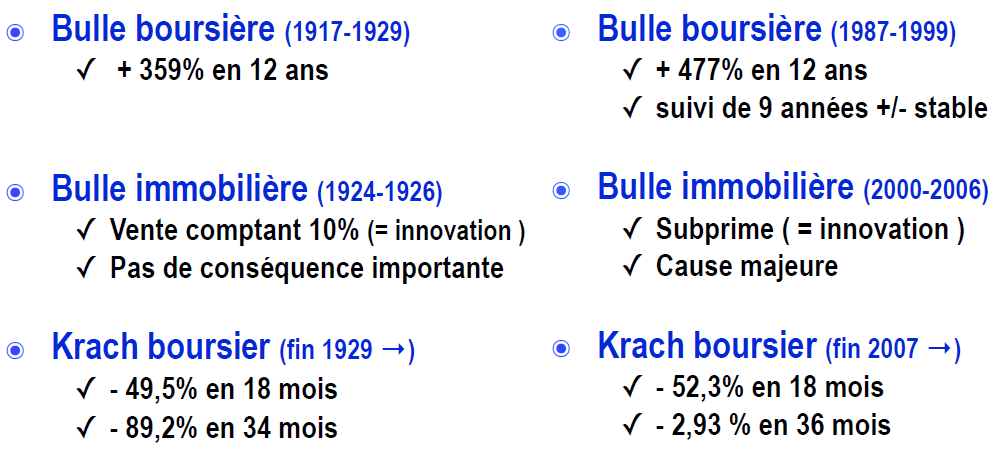
\includegraphics[scale=0.3]{43}
\end{wrapfigure}
\noindent On va établir ici les similitudes et les différences qui existent entre les crises de 1929 et de 2008. Le slide repris ci-contre est assez explicite. La seule chose à rajouter est que la première bulle immobilière (à gauche) concerne juste la Floride alors que la deuxième (à droite) concerne tout le pays ! 
\\\\
Les deux graphiques repris ci-dessous, représente le \textbf{Dow jones Industrial} (définition sur le graphique) pour des périodes reprenant les deux crises. \\
On peut voir sur le premier que l'économie ne se porte pas très mal entre 1946 et 2006, malgré une chute vers 2000. On voit que la bourse explose en raison des grosses spéculations de cette époque. \\
Sur le deuxième graphique, on reprend la période entre 1896 et 1936 (pour la crise de 29). On peut voir qu'à cette époque, la valeur de l'action n'est pas stable mais qu'à partir de 1925 on investit dans l'immobilier et donc on gagne bien. C'est là qu'à partir du 3 septembre 1929, on a le krach ! \\

\begin{minipage}{0.5\textwidth}
	\begin{flushleft}
		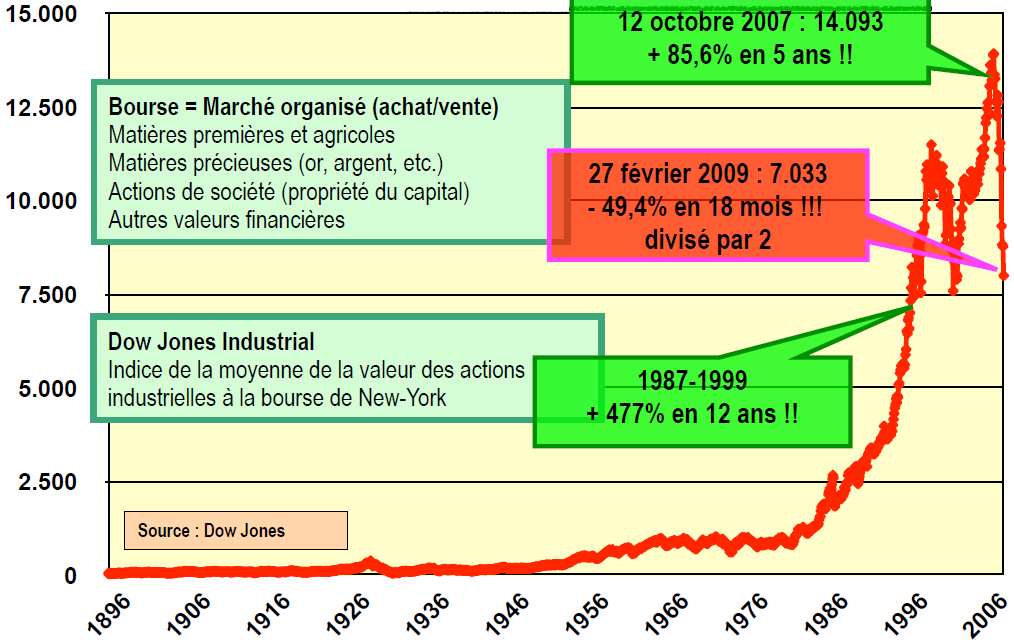
\includegraphics[scale=0.26]{44}
	\end{flushleft}
\end{minipage}
\begin{minipage}{0.5\textwidth}
	\begin{center}
		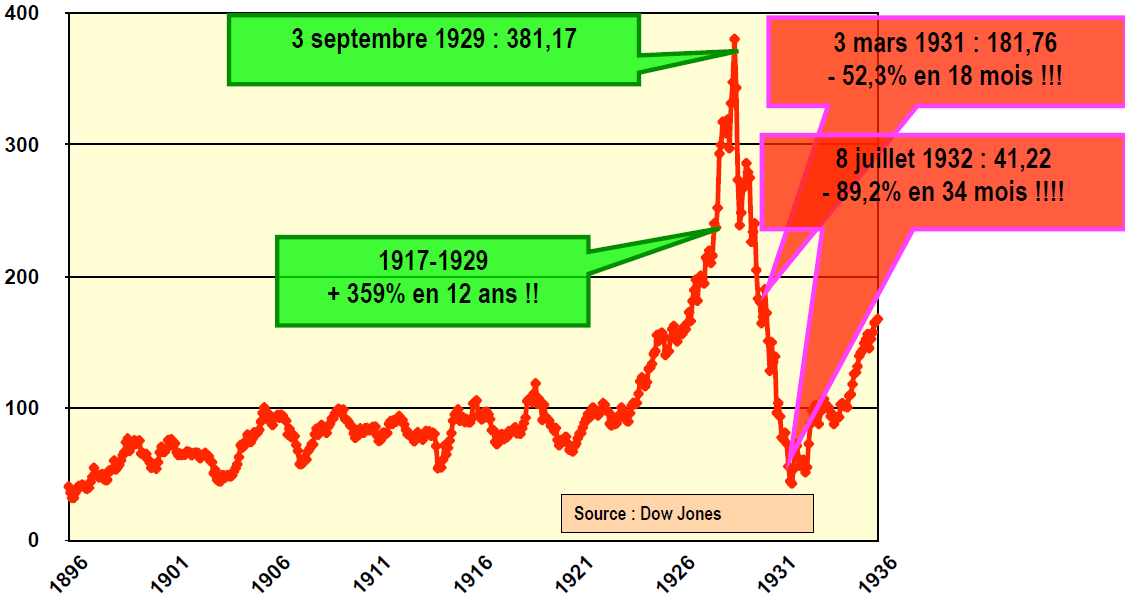
\includegraphics[scale=0.29]{45}
	\end{center}
\end{minipage}
\\
\begin{wrapfigure}[8]{l}{8.5cm}
	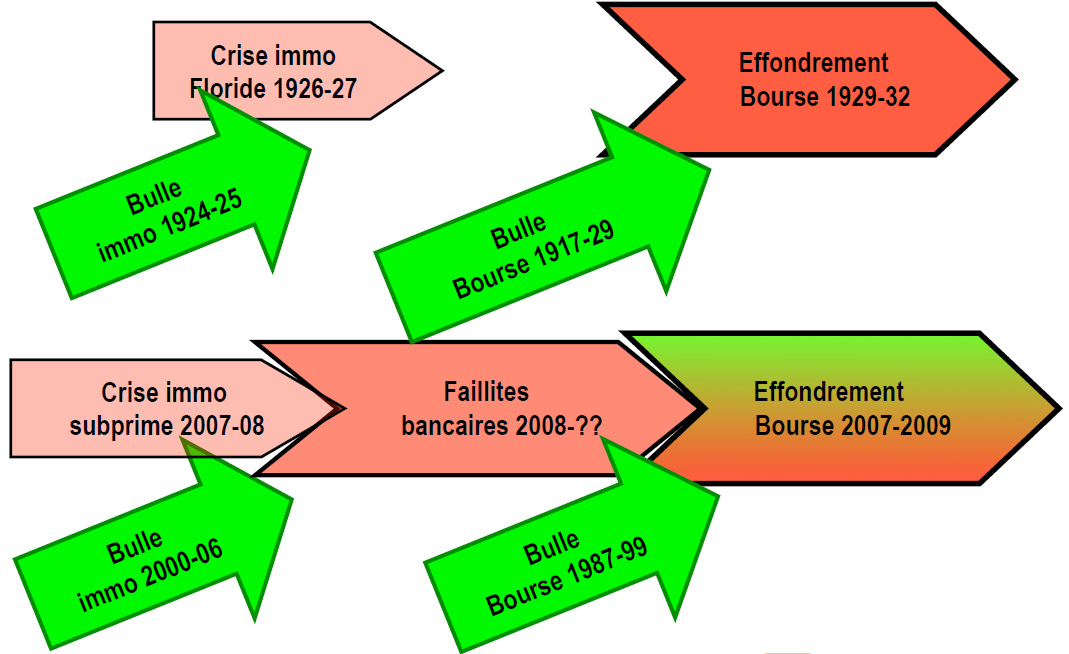
\includegraphics[scale=0.3]{46}
\end{wrapfigure}
\ \\ On peut cependant remarquer la grande similitude qu'il y a entre ces deux crises. En effet, on a toujours cette bulle économique avant l'effondrement. C'est ceci qui est illustré sur le graphique ci-contre. \\\\\\\\

\subsection{Innovations financières en 1929}
Tout d'abord, l'Europe avait besoin de réinvestir après la guerre donc il fallait des facilités. Les banques centrales d'Allemagne, France et UK demande a la Federal Reserve d'abaisser sont taux d'intérêt. Celui baisse le taux d'escompte\footnote{Taux d'intérêt auxquel la Federal Reserve prête aux banques.} à 3.5\%. Les banques ont donc accès facilement à l'argent et donc on peut prêter pour investir en bourse. \\
On a ensuite une innovation boursière, l'\textbf{achat d'actions sur marge}, qui consiste à effectuer des ventes inconditionnelles (pas compris, mail envoyé à Alle, attente de réponse) et de pratiquer l'effet de levier comme nous le connaissons dans les années 2000. \\
Ceci a eu pour conséquence l'esplosion des montants prêtés, mais aussi des taux (ils passent de 5\% à 12\% en 1928). Les banquiers font donc la fête (wouhou). 

\subsection{Bulle boursière}
Mais est-ce que c'est en raison de la croissance de l'économie qu'on a la bulle boursière ? Il faut savoir que la valeur des actions est le reflet des profits générés. En effet :

\begin{itemize}
	\item Si les profits croissent $\rightarrow$ dividendes payées $\rightarrow$ \textbf{hausse de la bourse}
	      	
	\item Si les perspectives de profit $\nearrow$ $\rightarrow$ anticipation de l'évolution $\rightarrow$ \textbf{hausse de la bourse}
\end{itemize}

Il est clair que si c'est le contreaire qui se passe, ça entraîne la baisse de la bourse. Pour mesurer les hausses justifié (si une action est rentable), on effectue le rapport cours de bourse / bénéfice (Price Earning Ratio). Ce dernier doit rester raisonable (moyenne entre 1881 et 2008 = 17). L'évolution de ce ratio est repris dans les deux graphiques qui suivent. Les étapes importantes sont indiquées dessus mais on peut dire que l'histoire se répète. \\

\begin{minipage}{0.5\textwidth}
	\begin{flushleft}
		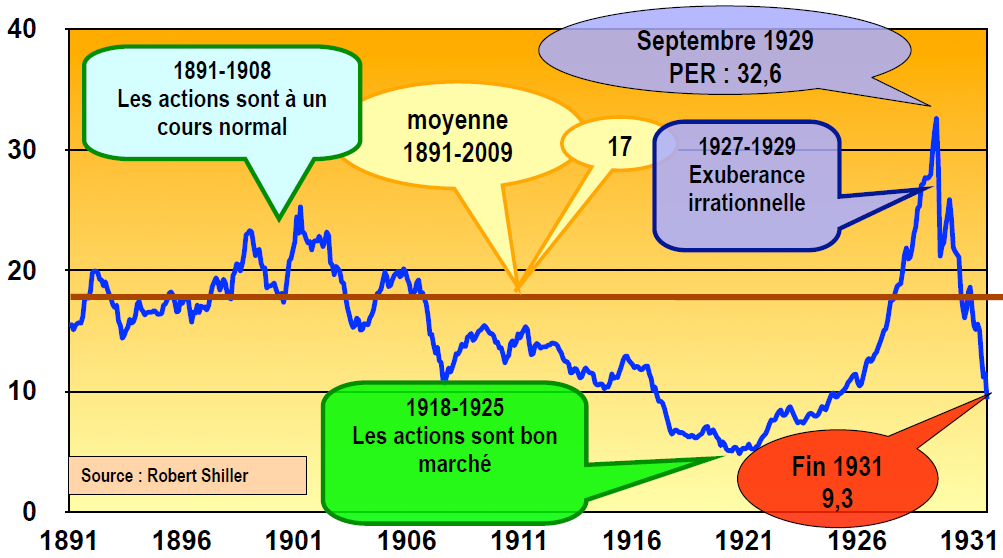
\includegraphics[scale=0.3]{47}
	\end{flushleft}
\end{minipage}
\begin{minipage}{0.5\textwidth}
	\begin{center}
		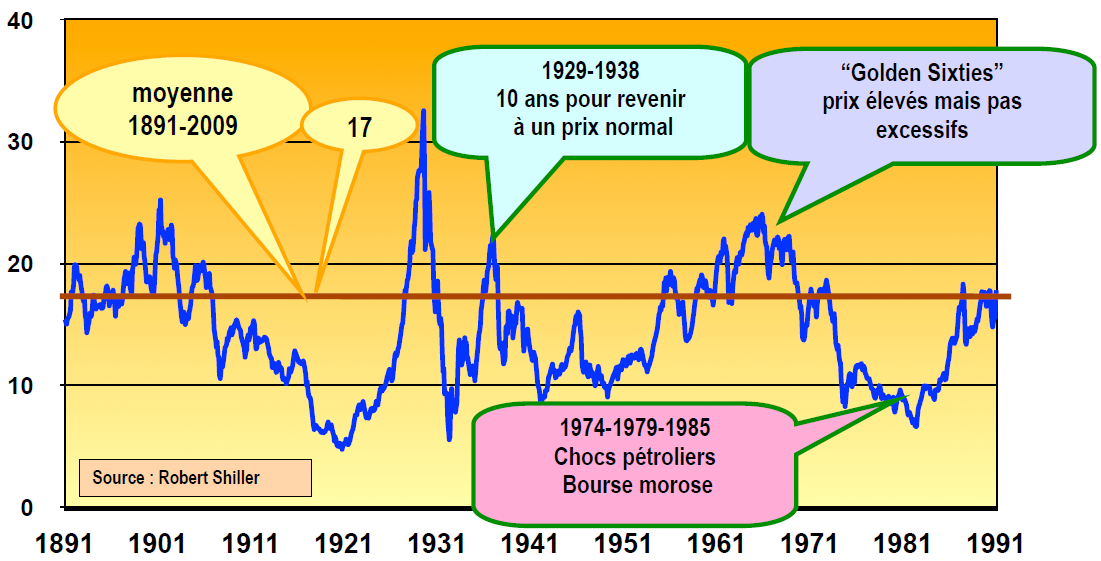
\includegraphics[scale=0.3]{48}
	\end{center}
\end{minipage}

\section{La crise de 1929}

\subsection{Cause}
Certaines grandes banques sont très créatives. Elles prêtent peu aux spéculateurs et créent des structures spéciales pour attirer leur argent. Elles ont aussi des structures de Trust d'investissement qui sont en fait des société spécialisé qui achètent des actions (en pratiquant l'effet de levier), ce sont les précurseurs des fonds actuels. Ces trusts d'investissement explose ! Leur nombre passe de 186 à 265 de 1928 à 1929.
\\\\
Cependant, certains d'entre eux prêtent aux spéculateurs. Du coup, quand la crise est arrivée, les spéculateurs ont perdu beaucoup. Il ne peuvent donc pas rembourser les banques qui perdent à leur tour. De plus, les épargnants perdent confiance et ça entraîne la faillite bancaire. Cependant, contrairement à aujourd'hui, l'Etat n'est pas intervenu. Donc, en même temps que les spéculateurs, les épargnant aussi ont tout perdu.

\subsection{Conséquences}
Ca a eu des conséquences mondiales puisque le commerce international a chuté en volume de -25\% entre 1929 et 1933 et -69\% en valeur (effondrement des prix) ! Ca a également comme conséquence direct, le chômage (12.8 millions de chômeurs aux USA en 1933, 6 en Allemagne et 4 en UK). Tout ceci a évidemment de lourdes conséquences sur le PIB des pays (graphique du PIB américain juste en bas). La deuxième figure est une comparaison entre les deux crises. On peut voir que les réactions ont été totalement différentes puisqu'en 1929 on a laissé la finance partir. Les conséquences sont donc beaucoup plus désastreuses pour 1929 puisque l'économie ne s'est pas remis pendant des années. Même les économistes de la Harvard Economic Society n'ont pas su voir clair. Il publiait tout le temps une remontée de l'économie entre 1929-30. \\

\begin{minipage}{0.5\textwidth}
	\begin{flushleft}
		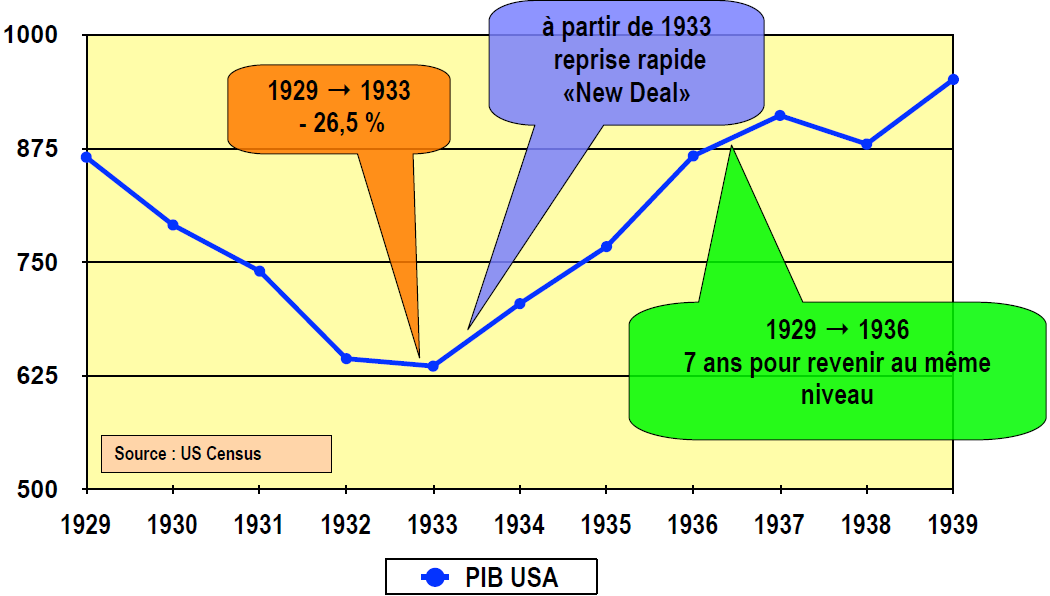
\includegraphics[scale=0.3]{49}
	\end{flushleft}
\end{minipage}
\begin{minipage}{0.5\textwidth}
	\begin{center}
		\includegraphics[scale=0.26]{50}
	\end{center}
\end{minipage}

\ \\

Pour finir, voilà la comparaison finale qu'on peut faire entre les deux crises. 

\begin{center}
	\includegraphics[scale=0.5]{51}
\end{center}

\section{Le rôle de la politique}
\subsection{Etat des lieux}
Différents hommes politiques ont joué de grands rôles en 1933. Parmi ceux-ci, on a F.D.Roosevelt, président américain entre 1933 et 1945 et qui a donc hérité de la crise de 1929. Il a permis de relancer l'économie. On a également Lloyd George, premier ministre anglais, qui a fait de même. \\
Si on revient en 1929, on se rappelle que la quasi-totalité des économistes n'a rien vu venir et d'autre ont nié la réalité de la dépression. De plus, à cette époque, on avait pas d'outil de statistique, on avait pas d'expérience de grande crise antérieure et on avait pas de modélisation économique \footnote{Liens entre les grandes données comme entre l'investissement et le produit national.}. On était donc penché sur l'économie à petite échelle et non sur l'économie dans son ensemble.

\subsection{Vision des libéraux}
Pour les libéraux, la base de l'économie c'est l'entreprise dont l'objectif doit être de maximiser le profit et de minimiser les coûts (notamment le salaire). La pensée était : Profits $\rightarrow$ Investissement $\rightarrow$ Emplois. Pour eux, il faut aussi que le taux d'intérêt suive l'épargne. De cette manière, les entreprises investiront. Cependant, en période de crise, ils ont tendance à diminuer les revenus, donc la consommation et aboutissent à une spirale négative. Donc il faut augmenter les revenus pour augmenter la consommation. 

\subsection{Le marxisme}
Même chose, l'entreprise est la base de l'économie. Ils éxagèrent même au niveau des salaires qui devaient appauvrir les salariés. La crise est bien vu parce que ça rétabli les profits. En effet, le chômage entraîne la baisse des salaires et la faillite d'entreprise fait diminuer la concurrence, donc le profit pour les restants monte. Tout se terminera bien sûr avec une grande crise. 

\section{John Maynard Keynes}
\subsection{Petite biographie}
C'est un homme qui a révolutionné les pensées libérales. Il était professeur à Cambridge et conseiller de l'Etat mais aussi conseiller en investissements financiers. Il s'est fait connaître une première fois au \textbf{Treasury and Peace Conference} pour la discussion des domages de guerre sur l'Allemagne. Il était clairement opposé (l'argent devait rester en Allemagne pour ne pas tuer l'économie). Il a joué un rôle important dans les crises des années '20 et '30. 

\subsection{La crise}
Lui non plus n'a pas vu arriver la crise. Il était très confiant en 1926 mais en 1928 il est très pessimiste quant à la crise. Il pense que la bulle financière américaine n'est pas basé sur la réalité de l'économie et que les prêts pour action (collateral loans) constituent un danger. Cependant, il se trompe en tant qu'investisseur financier \footnote{Son portefeuille financier passe de 44000 à 7815 en 2 ans !} alors qu'il est un très bon conseiller. \\
Mais Keynes perçoit aussi les conditions d'équilibre de l'économie. Les trucs importants sont : 

\begin{itemize}
	\item \textbf{La demande globale}
	\item \textbf{L'anticipation des entrepreneurs} sur la décision investir et donc, sur la demande globale 
	\item \textbf{L'anticipation des consommateurs} sur la décision d'épargner, donc de consommer et sur la demande globale. 
	\item \textbf{Du taux d'intérêt} sur la décision d'investir 
\end{itemize} 

\subsection{Modèle simple de l'économie}
\begin{wrapfigure}[7]{l}{9 cm}
	\includegraphics[scale=0.3]{52}
\end{wrapfigure}
De cela découle différents modèles de l'économie dont celui-ci. On a une boucle fermé qui montre que les ménages et les entreprises sont fortement liés. Le schéma est bien représentatif et aucune information supplémentaire n'est nécessaire. \\\\

\begin{wrapfigure}[5]{l}{9 cm}
	\includegraphics[scale=0.3]{53}
\end{wrapfigure}
On peut voir plus clairement sur ce schéma là que l'équilibre de l'économie serait permise si la totalité de l'épargne était investit en entreprises. Ce n'est bien sûr pas très réaliste.  \\\\\\\\\\\

\section{Modèle réaliste de l'économie}
\begin{wrapfigure}[9]{l}{9 cm}
	\includegraphics[scale=0.3]{54}
\end{wrapfigure}
Un modèle réaliste serait celui-ci puisque toutes les fuites et injections sont représentées. On a donc en plus du côté ménage les impôts et les importations et du coté entreprise on a que du bon, les investissements (les banques prêtent aux entreprises), les dépenses publiques (injectées par l'Etat) et les exportations. \\\\

\subsection{Consommation et épargne}
Penchons-nous d'un peu plus près sur ces deux termes. Le \textbf{revenu ($Y_d$)} des ménages consiste en le revenu du travail (salaires, ...), revenu du capital (actions, ...), les transferts (allocations familiales, chômage, ...) \textbf{mais} il faut retirer de cela le impots. \\
Le consommateur va partagerr son revenu en \textbf{consommation ($C$)} et \textbf{épargne ($S$)} : 
\begin{equation}
	Y_d = C + S
\end{equation}

Généralement, plus on gagne, plus la part de l'épargne augmente. On introduit donc la propension (part) moyenne du revenu consacré à la \textbf{consommation} comme étant $C/Y_d$ et celle consacré à \textbf{l'épargne} comme étant $S/Y_d$. \\
On va aussi introduire la \textbf{propension marginale} à consommer et à épargner (si on touche un euro en plus qu'est ce qu'on en fait) comme respectivement $\Delta C/\Delta Y_d$ et $\Delta S/\Delta Y_d$.

\subsection{Lien entre consommation et revenue}
On a observé empiriquement que la consommation évoluait linéairement avec le revenu. On a donc, avec des constantes $a$ et $b$ :

\begin{equation}
	C = a + b \cdot Y_d 
\end{equation}

La \textbf{propension marginale à consommer} (variation de la consommation) est donné par $C' = b$. La \textbf{propension moyenne à consommer} est alors donné par 

\begin{equation}
	\frac{C}{Y_d} = \frac{a}{Y_d} + b
\end{equation}

En remplaçant C par sa nouvelle expression

\begin{equation}
	S = Y_d - C = Y_d(1-b) + a
\end{equation}

Pour faire le compte des entreprises, on a comme entré d'argent la consommation, l'investissement (I), les dépenses publiques (G) et les exportations (X) et en argent perdu il y a les importations (M) : 

\begin{equation}
	AD = C + I + G + X - M
\end{equation}

Pour faire évoluer la demande globale, on peut agir sur chaque composante. On cherche donc une relance en cas de dépresson et un ralentissement en cas de surchauffe. \\
Le plus facile est d'agir sur les \textbf{investissements} car ce sont des décisions directes pour le public et il suffit de faire varier les taux d'intérêt au niveau privé. \\
On peut également jouer sur la consommation en réduisant les impôts et en ajoutant des allocations spécifiques. 

\begin{wrapfigure}[10]{l}{9 cm}
	\includegraphics[scale=0.3]{55}
\end{wrapfigure}
On aboutit au graphique ci-contre qui représente en bas, le ménage et en haut l'entreprise. On considère que le ménage consomme et investit et donc que son épargne augmente encore plus avec le revenu. On considère également que l'entreprise dépense ce qu'il gagne. On remarque que l'intersection entre \textbf{l'équilibre} et la courbe E est atteinte lorsque $S = I$. Il faudrait donc que \textbf{l'épargne soit totalement investit}. 

\subsection{Rôle de la confiance}
\begin{wrapfigure}[9]{l}{9 cm}
	\includegraphics[scale=0.3]{56}
\end{wrapfigure}
Nous sommes maintenant en plein \textbf{paradoxe de la prévoyance}. Mettons-nous dans le cas où c'est la crise économique et que tout le monde augmente sont épargne par prévoyance. Ceci entraîne la remontée de la courbe et on voit qu'on croise la courbe des revenus à 300 et plus à 400. Le revenu a donc baissé de 100 ! 

\section{Multiplicateur de l'investissement}
C'est la découverte majeure de Keyne. Le principe est qu'en injectant de l'investissement dans l'économie, on va créer du revenu supplémentaire. Intuitivement, \\
$
\mbox{Plus d'investissement} \rightarrow \mbox{plus de production} \rightarrow  \mbox{plus d'emploi} \rightarrow \mbox{plus de revenu} \rightarrow \mbox{plus de consommation} \\ \rightarrow \mbox{confiance en l'avenir} \rightarrow \mbox{les entreprises investissent} \rightarrow \mbox{cercle vertueux !}
$ \\
On peut aussi voir que sur le dernier graphique, si on fait monter la barre I, le revenu augmente. \\
Il persiste néanmoins un problème car le risque de fuite est élevé. En effet, si un Etat relance seul son économie par l'investissement public, on achètera à l'étranger, ce qui augmente les importations et on perd une partie importante du multiplicateur. Pour résoudre ce problème, on ferme les frontières aux importations. Cependant, si les autres pays ferment également leurs frontières, il y aura moins de concurrence et donc les prix monteront. 

\section{Le "New Deal"}
L'objectif de ce "nouvel accord" est de sortir de la grande dépression. Pour cela, il fallait \textbf{soutenir les plus pauvres} (assitance sociale, aides par le travail, Social Security System), \textbf{réformer les marchés financiers} (contrôle bourse et banques) et \textbf{relancer la demande globale} (investissement, consmmation des plus pauvres). \\
On a également \textbf{lutter contre le chômage} en payant des indemnités de chômage et en remettant les chômeurs les plus jeunes au travail, fait \textbf{des grands travaux} (électrification, routes), crée un système de \textbf{protection sociale} notamment la retraite et on a introduit des \textbf{libertés syndicales}. \\
Le résultat est \textbf{40 ans de stabilité et de croissance économique}. On termine le chapitre avec un résumé des idées de Keynes ci-bas. \\

\includegraphics[scale=0.5]{57}
	%%%%%%%%%%%%%%%%%%%%%%%
%%      Lecon 6      %%
%%%%%%%%%%%%%%%%%%%%%%%

\chapter{Mondialisation et délocalisation}
\section{Les faits}
\subsection{Contexte}
L'histoire commence dès 1968 avec la création de Dacia en Roumanie. C'est une entreprise crée sous régime communiste et est donc propriété de l'Etat. Cependant, ils achetaient le savoir-faire (les licences) à Renault. Ils avaient donc un retard technologique par rapport à l'Europe. \\
Ensuite, on a la chute du communisme en 1989 qui entraîne la chute accélérée de Dacia. Renault décide alors d'acheter l'usine déjà existante Dacia (Brownfield) en 1999 pour un prix minime. Ils ont pour objectif de  produire à bas coût des véhicules low cost. Ils visaient principalement les pays émergents, en comencant par la Roumanie. 

\subsection{Modernisation}
Ils ont eu un gros succès malgré les suspicions. A l'acquisition, l'usine éait obselète et la mentalité des ouvriers et des cadres ne correspondaient pas à la production moderne. VW fait pareil avec Skoda en Slovaquie. Ils vont donc introduire des standards européen avec une meilleure qualité de vie. Cependant, on a pas besoin de remplacer la main d'œuvre par des machines puisque ça coûte que dalle. \\
On augmente ainsi la productivité des usines en formant le personnel et en réorganisant le travail qui était très mal structuré. On arrive à doubler la production. Si le nombre d'effectif diminue de moitié et que la production double, alors la productivité quadruple.\\
On recherche de nouveaux modèles plus simple que la gamme classique pour le marché roumain, mais aussi pour l'exportation. On arrive ainsi à baisser le coût de production.

\subsection{Premier modèle}
La \textbf{Logan} est le premier nouveau modèle de Dacia. Les caractéristiques techniques restent très simples et mais la voiture est assez robustes (les routes sont mauvaises dans les pays émergents). On a pas d'électronique. Elle fonctionne à l'essence de qualité médiocre et on utilisera des vieux composants de Renault et Nissan. Elle n'est donc pas bonne pour l'environnement mais les crash-test restent correctes.\\
Ce modèle est deux fois moins cher que l'équivalent Renault ! On produit d'abord en Roumanie puis au Brésil et Maroc (Renault), ensuite, Mexique (Nissan), Iran et Russie (Lada).

\subsection{Résultats}
La Logan rencontre un grand succès dans les pays de l'est, surtout en Roumanie. En Europe de l'ouest aussi, même si au départ Renault ne voulait pas en vendre en Europe occidentale. \\
Depuis l'acquisition, Dacia est en perte. Après, elle fait du bénéfice (2005). Et à partir de 2011 ça devient la plus grosse marge du groupe Renault (30\% des ventes de Renault). \\
Pour ce qui est de la recherche, c'est en France qu'elle se passait à la base. A partir de 2011, on développe en Roumanie avec des ingénieurs roumains (premier modèle : Duster).

\section{Low cost}
\subsection{Mouvement irréversible ?}
La plupart des observateurs ont un point de vue positive. Mêmes les riches sont devenus de plus en plus attentifs aux prix parce que les revenus des ménages sont de plus en plus faible. Cependant, on veut quand même avoir un bon standard de vie avec un véhicule.\\
De plus, la concurence augmente et on a l'ouverture des marchés (libéralisation). La mondialisation permet donc de faire des productions à bas coût et de gagner une place importante dans cette concurrence.

\subsection{Ecarts salariaux}
\begin{wrapfigure}[10]{l}{8 cm}
\includegraphics[scale=0.3]{58}
\end{wrapfigure}
Le plus gros avantage de la délocalisation est la présence d'une main d'oeuvre à très bas coûts. On voit que dans les pays développé, le coût est assez haut en raison de toutes les sécurités sociales. Dacia paye quand même 20\% en plus que le coût moyen et avec les contremaître ça monte à 36\%. Ceci est dû au fait que Dacia a du former ses ouvriers au départ. 
\\
On observe quand même que les salaires en Roumanie, Chine et Vietnam augmentent assez vite. On remarque aussi que plus les salaires sont bas plus ils augmentent vite (+16\% de 2010 à 2012 en Roumanie).
\\\\
Dans les fondamentaux de la pensée économique on a \textbf{Adam Smith}, philosophe et économiste écossais. Il est le maître de la pensée classique du libéralisme économique. Il a dit : \textbf{« Il est prudent de ne jamais essayer de faire chez soi la
chose qui coûtera moins à acheter qu’à faire »}. Ca ne sert donc à rien de faire soi même quelque chose, si dans une autre zone géographique on la fait mieux. Faisons ce que nous faisons de meilleurs (meilleur accès aux matières premières, savoir faire, coûts de production plus bas).

\section{Renault au Maroc}
\subsection{Dacia Bis}
Dacia a bien réussi en Roumanie. Renault va cette fois essayer au Maroc aussi. Ils ouvrent une nouvelle usine à Tanger. A l'inverse de la Roumanie là on construit une usine de zéro (greenfield), très grande. Et on produit un nouveau véhicule (Lodgy). Si le marché primaire est le Maroc on veut surtout pouvoir vendre en Europe. \\
Les salaires sont bien plus bas qu'en France, mais on arrive à atteindre 75\% de productivité par rapport à la France. Cette fois on utilise les robots pour avoir une qualité élevée. Cela déclenche des réaction politique très fortes en France !

\subsection{Réactions politiques}
Les politiques, de droite, gauche et d'extrême ont tous le même point de vue. Il ne faut pas que Renault se dirige vers le low cost mais qu'il monte en gamme (Bruno Le Roux) et qu'il produise à l'extérieur des voitures destinées à la France et l'Europe (Christian Estrosi). Louis Aliot (numéro 2 du FN) veut carrément un protectionnisme européen. \\
De l'autre côté, le patron de Renault défend son cas. Il explique que ce n'est pas au détriment de la France. Ca permet de rajouter de l'ingénieurie en France. Les moteurs et la conception sont fait en France. On localise en France les produits les plus sofistiqués. "Si je veux faire du low-cost je ne peux pas le faire en France". De plus, la concurence n'est pas présente puisque Dacia et Renault ont des clients totalement différents. \\
Selon une opinion de syndicat, on se plaint de l'immigration et là c'est l'occasion d'offrir aux étrangers du travail dans leur pays. 

\section{Bénéficiaires et victimes}
Ce sont bien sûr les étrangers qui profitent. Ils ont un meileur revenu et une formation, un déloppement. Les consommateurs Européens aussi en profitent, car le prix est moindre. Les producteurs de matières premières aussi en bénéficient puisque la demande augmente, ainsi que les prix. \\
Par contre, les travailleurs non qualifiés des pays développés sont mal. 

\section{Innovations technologiques}
Tout d'abord, dans quel sens cela fonctionne ? 

\begin{itemize}
	\item Le progrès du bien-être humain est-il la conséquence du progrès technologique et de la croissance économique ? 
	
	\item Le progrès technologique est-il la cause de la croissance économique et la conséquence de la croissance économique ? 
	
	\item Le progrès technologique a-t-il des conséquences négatives sur la croissance économique et sur le bien-être humain ?
\end{itemize}

\subsection{Choix technologiques}
Par definition, les ressources sont rares. On a le travail, les machines, (travail passé rendu efficace), la terre, l'espace disponible et les matières premières. Jusqu'à présent, les gens veulent consommer plus que ce que l'économie peut produire. On va donc choisir ce qu'on va produire. 

\begin{wrapfigure}[9]{l}{8 cm}
\includegraphics[scale=0.3]{59}
\end{wrapfigure}
L'exemple classique des économiste est la comparaison entre le beurre et le canon. On conceptualise la production de bien de luxe et de première nécéssité. Ce qu'on fait, c'est qu'on va se placer tout le temps en dessous de la courbe max (en bleue) pour ne pas aller à la limie de l'économie. Mais comment aller plus loin en déplaçant cette courbe ? On peut ne rien changer aux technologies en montant la main d'œuvre. Pour cela, on fait amener des travailleurs émigrés. Ou alors, on peut aussi avoir plus de machines, mais pour ça, on va devoir faire des investissements. \\
Le second cas serait en abscence de changement des facteurs de production. Il faudrait alors une meilleure mise en oeuvre de ces facteurs (avancée technologique). On passe dans l'un ou l'autre cas à la courbe verte. 

\section{Innovations}
\subsection{Innovations radicales}
On introduit petit a petit les progrès technologiques. Mais on a parfois des progrès qui entraînent des changements en profondeur des conditions de vie ou de production. On appelle ça les innovations radicales. Avec ces changements, la hausse très forte de la productivité entraîne la baisse de certains prix. On a également de nouveaux biens ou services. Cela fait apparaître donc de nouveaux besoins. En voici quelques exemples : 

\begin{itemize}
	\item La machine à vapeur $\rightarrow$ remplace l’énergie humaine ou animale $\rightarrow$ très forte hausse de productivité et très forte baisse du prix du transport.
	
	\item Le transistor $\rightarrow$ le développement de l’électronique $\rightarrow$ nouveaux produits : télévision, ordinateurs, téléphones portables $\rightarrow$ très forte baisse du coût du traitement de l’information.
	
	\item La péniciline $\rightarrow$ augmentation de l'espérance de vie.
	
	\item Production à la chaîne $\rightarrow$ amélioration importante de la productivité.
	
	\item « Do it yourself » $\rightarrow$ amélioration importante de la productivité du travail rémunéré
\end{itemize}

\subsection{Révolutions industrielles}
\textit{C'est un changement radical du système technico-économique, un ensemble lié d’innovations radicales provoquant un saut de productivité dans la plupart des secteurs
de l’économie.} \\
Les facteurs de déclenchement sont : l'innovation permettant de diminuer vite et fort le prix d'un facteur clé, la disponibilité illimitée des inputs et un large  potentiel d'utilisation. Les deux tableaux ci-dessous reprennent les 5 révolutions industrielles. \\

\begin{minipage}{0.5\textwidth}
	\begin{flushleft}
		\includegraphics[scale=0.26]{60}
	\end{flushleft}
\end{minipage}
\begin{minipage}{0.5\textwidth}
	\begin{center}
		\includegraphics[scale=0.29]{61}
	\end{center}
\end{minipage}
\\\\
Si on regarde les 5 révolutions, elles ont toutes la conditions de la disponibilité illimité du facteur de production (coton, charbon, ...). Il faut également des entrepreneurs innovateurs qui vont porter le progrès loin : 

\begin{itemize}
	\item 3ème révolution : Siemens, Solvay, Marconi, Edison, Eastman
	\item 4ème révolution : Ford
	\item 5ème révolution : Steve Jobs, Bill Gates
\end{itemize}

\section{Facteurs influançant le développement technologique}
\subsection{Condition nécéssaire mais pas suffisante}
\begin{wrapfigure}[11]{l}{10 cm}
\includegraphics[scale=0.35]{62}
\end{wrapfigure}
Pour stimuler l'innovation, il faut la capacité de former les populations, être capable de développer de la recherche (éducation). La culture doit stimuler la créativité et l'originalité pour permettre les nouveautées. Il faut faire en sorte de traduire le développement en des produits et services concrets (acceptation des risquess et présence des moyens financiers). Finalement, le cadre légal doit stimuler l'innovation et l'entreprise.  

\subsection{Et demain ?}
\begin{wrapfigure}[12]{l}{10 cm}
\includegraphics[scale=0.35]{63}
\end{wrapfigure}
Dans la poursuite de ce qu'a rendu possible le transistor, l'innovation se poursuit dans la télécommunication mobile. On a accès très vite à de l'information pour un prix dérisoire. Nouveaux besoins : échange d'informations. Les performances des matériaux continueront à s’améliorer le contenu en énergie va continuer à diminuer et le taux de recyclage va augmenter considérablement. Par ailleurs, le contenu en information va continuer à augmenter. La vitesse de calcul, le volume stockable et transportable augmente, les produits sont adaptés aux besoins, communautés virtuelles, conséquences culturelles (facebook), ... 
\\\\
L’innovation technologique influencera encore plus
l’économie puisque la vitesse de changement et de transmission de l'innovation sera plus grande. Aussi, l'économie influencera encore plus l'innovation puisqu'il y a de plus en plus de concurrence entre les entreprises. 


	% %%%%%% %
% Chapitre 7 %
% %%%%%% %

\chapter{Le low cost et l'avenir de l'industrie en Europe}
\section{Entreprises low cost}
le low cost est intervenu comme une \textbf{rupture} du modèle économique traditionnel. En effet, si nous prenons le cas de Dacia, la grande innovation à été de se dire qu’au lieu d’avoir un but technologique (ingénieur qui recherche la pointe), on va se fixer un objectif en coût bas et on va se débrouiller pour qu’elle coute autant. On est passé du "design to cost" au "cost to design". D'autres comme Ryanair qui adoptent ce nouveaux modèles en réponse aux bas salaires et les inégalités (il ne faut pas renoncer à la consommer), sont également perçus comme rupture de modèles traditionels. \\
On a également des nouveaux modèles de consommation comme le partage, la location, le troc, les échanges etc. On passe donc du B2B \footnote{Business to comsumer} au C2C \footnote{Consumer to consumer (interaction entre clients)}. En réponse à cela, les traditionnels tendent à protéger leur modèle. 

\subsection{Ryanair}
Avant chaque pays avait sa compagnie national et chaque pays deservait les aéroports de son pays. Par la suite, des accords avec les autres compagnies ont permis d'élargir les réseau à l'international.
On va repenser le modèle de A à Z :
\begin{enumerate}
	\item On va quiter les grands aéroports pour aller vers les régionaux qui peuvent rapporter des subsident régionaux, sont plus rapides et plus simples.
	      	
	\item Les frais de l’industrie aéronautique sont très élevés, c’est pour ça qu’on va essayer de faire embarquer les gens plus rapidement et avoir une rotation élevé des vols \footnote{Aterissage/décollage}.
	      	
	\item On transporte plus de clients avec plus de siège (espace réduit).
	      	
	\item On simplifie l’accès aux billets grâce à internet et on réduit la possiblité de choix à un seul (classe éco uniquement)
	      	
	\item Avoir un taux de remplissage élevé (en 2014 on a 85\% des sièges occupés) Au plus c’est rempli au mieux c’est.
	      	
	\item Cout salariaux faible : on paye moins le personnel qui est souvent bien jeune et la législation sociale irlandaise est plus favorable.
\end{enumerate}

Tout cela permet à Ryanair de devenir en 2014 la première compagnie (en nombre de passagers) et d'être la marque la plus connue des européens. 

\subsection{Ikea}
Ikea un peu différent. On va innover, délocaliser et intégrer. Depuis le début, il y a 60 ans, c’est un innovateur. Il utilise systématiquement des nouveaux matériaux moins chers. De plus, au lieu de vendre des meubles montés, on doit apporter de soi même (assemblage et transport).\\
C'est aussi le roi de la délocalisation. C’est sûr qu’on trouve des produits de haut de gamme (italie, suisse) mais la plupart des produits viennent de l’europe de l’est et Asie. \\
Finalemenr, les fournisseurs sont intégrés dans la chaine de production, c'est à dire que ces fournisseurs sont indépendants mais travaillent comme si ils étaient liés à IKEA. Ils travaillent donc en fontion de la demande. \\ 
On a un concept nouveau aussi, c’est que les produits sont mondiaux et donc les catalogues de vente uniques.

\subsection{Free Mobile} 
C'est un opérateur téléphonique français. Sont but est de briser l’oligopole. En effet, on a peu de fournisseurs sur le marché qui s’arrangent pour ajuster les prix. Ca a pour conséquence que les prix sont élevé. Et en 2012 free mobile a obtenu la 4e licence d’opérateur et à la différence des autres, free se dit que je vais utiliser le réseau existant (celui de Orange). Free a démarré en annonçant une baisse des prix de 60 a 80\% (communication importante). Mais ce qui se fait ressentir au niveau des consommateurs c’est 40\% et en réalité la baisse n'a été que de 20 à 40\%. On a donc fortement jouer sur la communication pour attirer les clients. Les grands ont bien sûr dû réagir pour essayer de garder leur marché.\\
En 2014, Ils avaient 12\% du marché téléphonique. On estime qu’il y a eu une perte d’emploi de 30 000 à 50 000 (vu qu’il y a moins de cout). SFR a été vendu à Numéricable, ce qui est signe d'un remodelage du secteur. 

\newpage 
\section{Pourquoi le low cost ?}
\begin{wrapfigure}[11]{l}{9.5 cm}
	\includegraphics[scale=0.3]{64}
\end{wrapfigure}
\noindent Tout d'abord, on remarque qu'il y a une proportion de bas salaire qui est devenu plus importante qu’avant. On mesure ceci grâce au salaire médian. 50\% de la population gagne un salaire plus grand et et exactement 50\% des salaires plus bas sont gangés par l'autre moitié. On remarque que la Belgique est un peu moins bien que la Suède mais est la plus égale au niveau des salaires. Pour clarifier, pour la pologne, 24\% des gens qui ont moins de 66\% du salaire médian (donc dans tous les salarié la moitié des gens gagne moins que ce salaire et la moitié gagne plus et on prend 66\% de ce salaire).

\begin{wrapfigure}[10]{l}{9.5 cm}
	\includegraphics[scale=0.3]{65}
\end{wrapfigure}
\ \\
Autre manière de mesurer, c’est une mesure fait en France du niveau de vie moyen des 10\% des francais qui gagne le plus par rapport au 10\% des francais qui gagne le moins. En 1996 Les plus riches gagnaient 6 fois ce que les pauvres gagnaient et maintenant on est a 7,5 fois.\\\\
On ne souhaite malgré tout pas renoncer à consommer. Les standards de vie s’élève : télévision et publicité, présence de centre commerciaux partout et présence de temps libre. Tout cela incite les gens à consommer. D'où la raison pour laquelle le low cost marche bien.

\section{Nouveaux modèles de consommation}
\subsection{Partage, location, troc, ...}
\subsubsection{Airbnb}
On en a discuté dans l'intro au chapitre. Puisque les moyens sont en baisse, on trouve de nouveaux moyens de consommer. \\
On a par exemple Airbnb qui est disponible grâce à internet et dont le concept est "Partage et location de bed \& breakfeast" entre particuliers. Et c’est beaucoup moins cher que les hôtels. 

\subsubsection{Cambio}
On a aussi Cambio (voitures partagées). On commence à voir que le pourcentage de jeune génération propriétaire d’une voiture diminue. On renonce à la propriété et on partage des véhicules. Pas encore fameux au niveau utilisation.

\subsubsection{Carpooling.com}
Ca va encore plus loin que le carsharing, c’est le covoiturage (utiliser la voiture de qq d’autre pour se déplacer). C'était déjà fortement à la mode dans les années 70' avec les prix élevés de carburants et là ça revient en force avec l'arrivée d'internet. C'est un concurrent direct pour les moyens de transport actuels puisqu'il se fait aussi à grande distance (trains, avions, bus).

\subsection{Du B2C au C2C}
Le marché traditionnel consiste en l’entreprise qui vend au consommateur. Les nouveaux marchés permettent aux consommateurs de vendre à d'autres consomateurs. On est donc plus du côté du produit recyclé que du produit nouveau. Et grâce à internet, tout cela est plus facile puisqu'on a pas besoin de marché physique. On a par exemple eBay (ventes entre particuliers), Trocheures.fr (échange de service bricolage, tu fais ce que tu sais et moi je te fait ce que je sais).

\subsection{Réaction des modèles traditionnels}
On a diférentes réactions selon le secteur concerné :
\begin{itemize}
	\item Dans l'aérien, on converge vers les nouveaux modèles low cost (on augmente le nombre de vol, de siège, utilisation de internet). Alors que les low cost évolue vers le traitionnel afin d'augmenter leur profit.
	      
	\item Défense : TGV commence à diminuer et non a stagner donc on estime que l’impact le plus important de  baisse c’est le covoiturage. 
	      
	\item Les consommateurs change d’attitude de plus en plus vite et donc les entreprises doivent s’adapter de plus en plus vite. Le low cost garde une longueur d'avance. 
\end{itemize}
\newpage

\section{L'avenir de l'industrie en Europe}
\subsection{Evolution de l'emploi}
On ne parlera que de la Belgique. Signalons pour commencer que beaucoup de licenciements se sont opérés dans le secteur inustriel en Belgique (ex : Caterpillar, Heinz). 
\begin{wrapfigure}[11]{l}{9.5 cm}
	\includegraphics[scale=0.3]{66}
\end{wrapfigure}
\ \\
Pas qu'en Belgique aparemment puisque, malgré une baisse lente pendant assez longtemps, à partir de 2004 on a un véritable repli, notamment avec le UK qui a perdu 30\% d'emplois. Cas particulier de la Pologne qui doit sa hausse d'emplois à son intégration à l’UE. Tout ça correspond à 6 millions d'emploi perdus en 12 ans. 

\begin{wrapfigure}[12]{l}{9.5 cm}
	\includegraphics[scale=0.3]{67}
\end{wrapfigure}
\ \\
Sur cet autre graphe on représente la part des employés travaillant dans l'industrie. On à la barre horizontale qui représente la moyenne européenne. On peut remarquer que des pays comme la France et la Belgique sont bien en dessous et d'autres comme l'Allemagne et la Tchéquie sont bien au dessus. On remarquera qu'en générale la tendance a été une perte d'emplois dans le secteur. 

\begin{wrapfigure}[12]{l}{9.5 cm}
	\includegraphics[scale=0.29]{68}
\end{wrapfigure}
\ \\
On parle d’industrie mais c’est pas la même chose partout. On a de l’industrie beaucoup développé et d’autres bien plus basiques. On constate que les Pays-Bas ont peu d’emplois mais chaque emploi crée beacoup de valeur. Ils ont peu d’industrie mais des industries très pointues avec des gens qualifiés. La Belgique se porte bien aussi car chaque ouvrier crée plus de valeur que ceux de l’Allemagne. On est dans une série de pays ou on est au dessus de la moyenne. Par contre les pays où il y a beaucoup d’industrie, on a très peu de valeur parce que ce sont des industries assez classiques et rudimentaires. \\
La moyenne de la part de l'industrie dans le PIB en Europe avoisine les 20\% et à part l'Allemagne et la Suède pour qui cette part est légèrement montée, cette part a baissé et en France et Belgique cette part est très basse.

\subsection{Constats}
On a une très grande disparité en Europe avec des champions comme l’Allemagne où on retrouve l’automobile haut de gamme, la téléphonie ... Là où l’Europe est forte. Dans le sud et l’est on a des produit de valeur ajoutée pas trop élevée.\\
Selon l’endroit, on a soit déclin (pays de vieille industrie comme le Benelux), soit stabilité (Allemagne, Italie), soit croissance (Europe de l'Est) de l'emploi. V slide. La croissance des pays de l’est est dû a la délocalisation. \\
La walonie est un grand exemple de la ruine de l’industrie. Mais elle s'ensort actuellement avec l’aerospatial et l'aero qui sont des points très fort de la walonie, la pharmacie et le biotech également.

\section{Exemples d'industrie}
\subsection{Lego}
Je crois qu'on sait tous ce qu'est Lego et on a tous kiffé ça ... Design, simplification et mondialisation qui ont permis la réussite de cette entreprise, née en 1980, dans le jouet Leur grande force était la petite enfance mais ils ont perdu cette activité à partir de 1998. On s’est même posé la question de savoir si lego n'avait pas raté le tournant du 21è siecle. Differentes risons : se sont trop diversifié et se sont rendu trop complexe et ont donc eu difficile à gérer tout ça. //
On a eu des baisse d’emplois importante et ils se sont dit "on a perdu cette capacité a comprendre les enfants alors on va revenir à nos racines". Ils sont reparti aux fondamentaux. Ils ont changé des choses fondamentales et depuis 2004 on travaille avec des non créateurs. Ce sont des gens qui sont nettement moins marrants mais on était obligé.
On a mis une grande priorité sur l'Asie pour la délocalisation (2008). Chaque année on a crée des produits nouveaux et ça a marché. Le siège centrale est au dannemark à billund. 

\begin{wrapfigure}[7]{l}{9.5 cm}
	\includegraphics[scale=0.29]{68}
\end{wrapfigure}
Ils n’ont pas hésité à réduire le nombre d'employés avant de le remonter plus tard. A la base 100\% danoise puis ce sont implanté en Europe et le reste du monde. C’est un exemple réussi d’industrie mais qui a dû se remettre en question. 

\subsection{Audi Brussels}
On héberge toujours une très grande usine Audi. Ce qui a joué : gros sacrifice sociale et toujours travailler sur la qualité. Ieteren est un carossier bruxellois qui a donc débuter l'activité en 1949 en raison des droits d'importation élevés à la douane. Plein d’usines au départ. En 1975 on arrete la production de la coccinelle. Enorme croissance du groupe VW qui met en compétition ses différentes usines (vous devez etre bons en prix et en qualité). En 2005, le point positif de VW-Forest était la productivité, la qualité élevée et la localisation de l'usine (proche de frets). Fin 2005 VW récolte de mauvais résultats et décide d'une restructuration, notamment en fermant l'usine de Forest.

\subsection{SEB}
En mode fortement résumé : sacrifice sociale et qualité pour garder en vie cette société (Tefal, moulinex, krups). SEB fabrique toujours beaucoup en Europe et est protégé par des barrières technologiques. Il a massivement pratiqué l’externalisation de la production pour les bêtes produits afin de diminuer les coûts. L'entreprise mise beaucoup sur la recherche et l'innovation. 60\% des produits ont moins de 3 ans et l'équipe de recherche est assez développé. Différenciation du low cost en misant sur la sophistication (so sofisticated) et la simplicité d'usage. A partir de 2009 c'est surtout en dehors de l'Europe que les ventes ont augmentés. 

\subsection{Cardio3}
Une entreprise wallonne de biotechnologie parmi plus d’une centaine des plus grandes (GSK, UCB, IBA). 70\% de l'activité biotechnologique en Belgique ! $\pm$ 15.000 emplois industriels multiplié par 3 en 15 ans. Valorisation de la recherche universitaire. Spécialité : maladies cardiaques.

\section{Re-shoring et Back-shoring}
La mondialisation et off-shoring est une tendance longue. On observe une
délocalisation de l’industrie européenne totale ou partielle. Totale pour les
produits finis : textile, chaussures, meubles, électronique. Partielle : sous
-traitance : composants, prestations, informatiques, administration, call
centers. Pays émergents proches ou lointains. Proches : Méditerranée,
Europe de l’est. Lointains : Asie, Amérique du Sud, . . . Afrique. Causes :
Avantages compétitifs (Adam Smith) : Coûts salariaux (niveau de vie, 
protection sociale, etc.) et coûts de l’énergie et des matières premières.
Délocalisation n'est pas évitable et parfois c'est totale. \\
Certains reviennent petit à petit vers leur pays d'origine. Par exemple Apple qui a rouverte une ligne de production de macbook pro aux USA et BZ Moda pour les chaussures en Italie. La cause de ce retour ? Les couts salariaux dans les pays émergents sont en train de monter alors que ceux chez nous diminuent. On a une hausse de la productivité avec la même main d’oeuvre. On est capable de s'adapter plus rapidement à toute demande et bien sûr n'oublions pas l'image de marque favorisé avec le retour au pays. \\
L'ampleur de ce reshoring est difficile à mesurer mais voici un aperçu selon
le secteur : Textile et chaussures : 35\%, Mécanique, robotique : 20\%;
Mobilier : 15\%; Electronique : 10\%; Electro-ménager : 10\%.

\subsection{Les leçons d'Adam Smith}
Qu’est ce qu’on a de plus que les autres ? Main d’oeuvre très qualifié, recherche … Très développé, et proximité des marchés. Désavantage : cout de la main d’oeuvre. Ils faut utiliser nos qualité en stimulant la recherche et le développement.\\
\\
Si tu es arrivé jusque là félicitation !
	
	
	%%%%%%%%%%%%%%%%%
	% Bibliographie %
	%%%%%%%%%%%%%%%%%
	%\newpage
	%\chapter{Bibliographie}
	%\nocite{*}
	%\printbibliography[heading=none]
	
	%%%%%%%%%%%
	% Annexes %
	%%%%%%%%%%%
	\appendix
	%\chapter{Annexe 1}
Coucou
	
	
\end{document}
